% Options for packages loaded elsewhere
\PassOptionsToPackage{unicode}{hyperref}
\PassOptionsToPackage{hyphens}{url}
%
\documentclass[
  man,floatsintext]{apa6}
\usepackage{lmodern}
\usepackage{amssymb,amsmath}
\usepackage{ifxetex,ifluatex}
\ifnum 0\ifxetex 1\fi\ifluatex 1\fi=0 % if pdftex
  \usepackage[T1]{fontenc}
  \usepackage[utf8]{inputenc}
  \usepackage{textcomp} % provide euro and other symbols
\else % if luatex or xetex
  \usepackage{unicode-math}
  \defaultfontfeatures{Scale=MatchLowercase}
  \defaultfontfeatures[\rmfamily]{Ligatures=TeX,Scale=1}
\fi
% Use upquote if available, for straight quotes in verbatim environments
\IfFileExists{upquote.sty}{\usepackage{upquote}}{}
\IfFileExists{microtype.sty}{% use microtype if available
  \usepackage[]{microtype}
  \UseMicrotypeSet[protrusion]{basicmath} % disable protrusion for tt fonts
}{}
\makeatletter
\@ifundefined{KOMAClassName}{% if non-KOMA class
  \IfFileExists{parskip.sty}{%
    \usepackage{parskip}
  }{% else
    \setlength{\parindent}{0pt}
    \setlength{\parskip}{6pt plus 2pt minus 1pt}}
}{% if KOMA class
  \KOMAoptions{parskip=half}}
\makeatother
\usepackage{xcolor}
\IfFileExists{xurl.sty}{\usepackage{xurl}}{} % add URL line breaks if available
\IfFileExists{bookmark.sty}{\usepackage{bookmark}}{\usepackage{hyperref}}
\hypersetup{
  pdftitle={What measure of effect size using when performing a Welch's t-test?},
  pdfauthor={Marie Delacre, Daniel Lakens, Christophe Ley, Limin Liu, \& Christophe Leys},
  pdfkeywords={keywords},
  hidelinks,
  pdfcreator={LaTeX via pandoc}}
\urlstyle{same} % disable monospaced font for URLs
\usepackage{longtable,booktabs}
% Correct order of tables after \paragraph or \subparagraph
\usepackage{etoolbox}
\makeatletter
\patchcmd\longtable{\par}{\if@noskipsec\mbox{}\fi\par}{}{}
\makeatother
% Allow footnotes in longtable head/foot
\IfFileExists{footnotehyper.sty}{\usepackage{footnotehyper}}{\usepackage{footnote}}
\makesavenoteenv{longtable}
\usepackage{graphicx,grffile}
\makeatletter
\def\maxwidth{\ifdim\Gin@nat@width>\linewidth\linewidth\else\Gin@nat@width\fi}
\def\maxheight{\ifdim\Gin@nat@height>\textheight\textheight\else\Gin@nat@height\fi}
\makeatother
% Scale images if necessary, so that they will not overflow the page
% margins by default, and it is still possible to overwrite the defaults
% using explicit options in \includegraphics[width, height, ...]{}
\setkeys{Gin}{width=\maxwidth,height=\maxheight,keepaspectratio}
% Set default figure placement to htbp
\makeatletter
\def\fps@figure{htbp}
\makeatother
\setlength{\emergencystretch}{3em} % prevent overfull lines
\providecommand{\tightlist}{%
  \setlength{\itemsep}{0pt}\setlength{\parskip}{0pt}}
\setcounter{secnumdepth}{-\maxdimen} % remove section numbering
\shorttitle{Effect size}
\affiliation{
\vspace{0.5cm}
\textsuperscript{1} Université Libre de Bruxelles, Service of Analysis of the Data (SAD), Bruxelles, Belgium\\\textsuperscript{2} Eindhoven University of Technology, Human Technology Interaction Group, Eindhoven, the Netherlands\\\textsuperscript{3} Universiteit Gent, Department of Applied Mathematics, Computer Science and Statistics,4 Gent, Belgium}
\keywords{keywords\newline\indent Word count: X}
\usepackage{csquotes}
\usepackage{upgreek}
\captionsetup{font=singlespacing,justification=justified}

\usepackage{longtable}
\usepackage{lscape}
\usepackage{multirow}
\usepackage{tabularx}
\usepackage[flushleft]{threeparttable}
\usepackage{threeparttablex}

\newenvironment{lltable}{\begin{landscape}\begin{center}\begin{ThreePartTable}}{\end{ThreePartTable}\end{center}\end{landscape}}

\makeatletter
\newcommand\LastLTentrywidth{1em}
\newlength\longtablewidth
\setlength{\longtablewidth}{1in}
\newcommand{\getlongtablewidth}{\begingroup \ifcsname LT@\roman{LT@tables}\endcsname \global\longtablewidth=0pt \renewcommand{\LT@entry}[2]{\global\advance\longtablewidth by ##2\relax\gdef\LastLTentrywidth{##2}}\@nameuse{LT@\roman{LT@tables}} \fi \endgroup}


\usepackage{lineno}

\linenumbers
\usepackage{rotating}
\DeclareDelayedFloatFlavor{sidewaysfigure}{figure}
\usepackage{lscape}
\newcommand{\blandscape}{\begin{landscape}}
\newcommand{\elandscape}{\end{landscape}}

\title{What measure of effect size using when performing a Welch's t-test?}
\author{Marie Delacre\textsuperscript{1}, Daniel Lakens\textsuperscript{2}, Christophe Ley\textsuperscript{3}, Limin Liu\textsuperscript{3}, \& Christophe Leys\textsuperscript{1}}
\date{}

\authornote{

Correspondence concerning this article should be addressed to Marie Delacre, CP191, avenue F.D. Roosevelt 50, 1050 Bruxelles. E-mail: \href{mailto:marie.delacre@ulb.ac.be}{\nolinkurl{marie.delacre@ulb.ac.be}}}

\abstract{

}

\begin{document}
\maketitle

\hypertarget{intro}{%
\section{Intro}\label{intro}}

During decades, researchers in social science (Henson \& Smith, 2000) and education (Fan, 2001) have overestimated the ability of the null hypothesis (H0) testing to determine the importance of their results. The standard for researchers in social science is to define H0 as the absence of effect (Meehl, 1990). For example, when comparing the mean of two groups, researchers commonly test the H0 that there is no mean difference between groups (Steyn, 2000). Any effect that is significantly different from zero will be seen as sole support for a theory.

Such an approach has faced many criticisms among which the most relevant to our concern is that the null hypothesis testing highly depends on sample size: for a given alpha level and a given difference between groups, the larger the sample size, the higher the probability of rejecting the null hypothesis (Fan, 2001; Kirk, 2009; Olejnik \& Algina, 2000; Sullivan \& Feinn, 2012). It implies that even tiny differences could be detected as statistically significant with very large sample sizes (McBride, Loftis, \& Adkins, 1993)\footnote{Tiny differences might be due to sampling error, or to other factors than the one of interest: even under the assumption of random assignment (which is a necessary but not sufficient condition), it is almost impossible to be sure that the only difference between two conditions is the one defined by the factor of interest. Other tiny factors of no theoretical interest might slightly influence results, making the probability of getting an actual zero effect very low. This is what Meehl (1990) calls 'systematic noise'.}.

Facing this argument, it has become an adviced practice to report the \emph{p}-value assorted by a measure of the effect size, that is, a quantitative measure of the magnitude of the experimental effect (Cohen, 1965; Fan, 2001; Hays, 1963). This practice is also highly endorsed by the American Psychological Association (APA) and the American Educational Research Association (AERA) (American Educational Research Association, 2006; American Psychological Association, 2010). However, only a limited number of studies have properly reported effect size in the last decades.

Generally, there is a high confusion between the effect size and other related concepts such as the Clinical significance. Moreover, there are several situations that call for effect size measures and, in the current litterature, it is not always easy to know which measure to use in which context. We will therefore begin this paper with 3 sections in which we will:\\
1. Clearly define what is a measure of effect size;\\
2. List the different situations that call for effect sizes measures;\\
3. Define required properties of the effect size estimators depending on the specific situation.

Moreover, it is highly recommended to compute a confidence interval around the point effect size. In a fourth section, we will therefore summarize in how far it is an added value to mention the confidence interval around the effect size.

After these general adjustments, we will focus our attention on \enquote{between-subject} designs where individuals are randomly assigned into one of two independent groups and group scores are compared based on their means\footnote{We made this choice because *t*-tests are still the most commonly used tests in the field of Psychology.}. Because it has been widely argued that there are many fields in psychology where the assumption of equal variances between two populations is ecologically unlikely (Delacre, Lakens, \& Leys, 2017; Erceg-Hurn \& Mirosevich, 2008; Grissom, 2000), it is becoming more common in statistical software to present a \emph{t}-test that does not hold under this assumption by default, namely the Welch's \emph{t}-test (e.g., R, Minitab). However, similar issues for the measures of effect sizes have received less attention (Shieh, 2013), and Cohen's \(d_s\) remains persistent\footnote{For example, in Jamovi, Cohen's ds is provided, independently of whether one performs Student's or Welch's t-test.}. One possible reason is that researchers cannot find a consensus on which alternative should be used (Shieh, 2013). We will limit our study to the standardized mean difference, called the \emph{d}-family, because it is the dominant family of estimators of effect size when comparing two groups based on their means (Peng, Chen, Chiang, \& Chiang, 2013; Shieh, 2013), and we will see that even in this very specific context, there is little agreement between researchers as to which is the most suitable estimator. According to us, the main reason is that it is difficult, based on currently existing measures, to optimally serve all the purposes of an effect size measure. Throughout this section, we will:\\
1. Present the main measures of the \emph{d}-family that are proposed in the literature, related to the purpose they serve, and introduce a new one, namely the \enquote{transformed Shieh's \emph{d}} that should help at reaching all the purposes simultaneously;\\
2. Present and discuss the results of simulations we performed, in order to compare existing measures and our newly introduced one;\\
3. Summarize our conclusions in practical recommendations. In this section, we will provide useful tools (i.e., an R package) to compute relevant measures of effect sizes and related information.

\hypertarget{measure-of-effect-size-what-it-is-what-it-is-not}{%
\section{Measure of effect size: what it is, what it is not}\label{measure-of-effect-size-what-it-is-what-it-is-not}}

The effect size is commonly referred to as the practical significance of a test. Grissom \& Kim (2005) define the effect size as the extent to which results differ from what is implied by the null hypothesis. In the context of the comparison of two groups based on their means, depending on the defined null hypothesis (considering the absence of effect as the null hypothesis), we could define the effect size either as the magnitude of differences between parameters of two populations groups are extracted from (e.g.~the mean; Peng \& Chen, 2014) or as the magnitude of the relation between one dichotomous factor and one dependent variable (American Educational Research Association, 2006). Both definitions refer to the most famous families of measures of effect sizes (Rosenthal, 1994): the \emph{d}-family and the \emph{r}-family.

Very often, the contribution of the measures of effect size is overestimated. First, benchmarks about what should be a small, medium or large effect size might have contributed to viewing the effect size as a measure of the importance or the relevance of an effect in real life, but it is not (Stout \& Ruble, 1995). The effect size is only a mathematical indicator of the magnitude of a difference, which depends on the way a variable is converted into numerical indicator. In order to assess the meaningfulness of an effect, we should be able to relate this effect with behaviors/meaningful consequences in the real world (Andersen, McCullagh, \& Wilson, 2007). For example, let us imagine a sample of students in serious school failure who are randomly divided into two groups: an experimental group following a training program and a control group. At the end of the training, students in the experimental group have on average significantly higher scores on a test than students in the control group, and the difference is large (e.g.~30 percents). Does it automatically mean that students in the experimental condition will be able to pass to the next grade and to continue normal schooling? Whether the computed magnitude of difference is an important, meaningful change in everyday life refers to the interpretation of treatment outcomes and is neither a statistical nor mathematical concept, but is related to the underlying theory that posits an empirical hypothesis. This concept is sometimes called \emph{Clinical significance} (Grissom \& Kim, 2012; Thompson, 2002) or \emph{Social significance} (Tyler, 1931) in the current literature. However, in our conception, we should use a more general term and we propose to rename this concept to \emph{Applied significance}\footnote{In our conception Applied significance encompasses all what refers to the relevance of an effect in real life, such as for instance clinical, personnal, social, professionnal relevance.}.

Second, in the context of the comparison of two groups based on their means, the effect size should not replace the null hypothesis testing. Statistical testing allows the researcher to determine whether the oberved departure from H0 occured by chance or not (Stout \& Ruble, 1995), while effect size estimators allow to assess the practical signficance of an effect, and as reminds Fan (2001): \emph{\enquote{a practically meaningful outcome may also have occured by chance, and consequently, is not trustworthy}} (p.278). For this reason, the use of confidence intervals around the effect size estimate is highly recommended (Bothe \& Richardson, 2011), as will be explained in a later section.

\hypertarget{different-purposes-of-effect-size-measures}{%
\section{Different purposes of effect size measures}\label{different-purposes-of-effect-size-measures}}

Effect size measures can be used in an \emph{inferential} perspective:\\
- The effect sizes from previous studies can be used in a prior power analysis when planning a new study (Lakens, 2013; Prentice \& Miller, 1990; Stout \& Ruble, 1995; Sullivan \& Feinn, 2012; Wilkinson \& the Task Force on Statistical Inference, 1999);\\
- We can compute confidence limits around the point estimator (Shieh, 2013) in order to replace conventional hypothesis testing : if the null hypothesis area is out of the confidence interval, we can conclude that the null hypothesis is false.

Measures of effect size can also be used in a \emph{comparative} perspective, that is, to assess the stability of results across designs, analysis, samples sizes (Wilkinson \& the Task Force on Statistical Inference, 1999). This includes\\
- the comparison of results from 2 or more studies (Prentice \& Miller, 1990);\\
- the incorporation of results in meta-analysis (Lakens, 2013; Li, 2016; Nakagawa \& Cuthill, 2007; Stout \& Ruble, 1995; Wilkinson \& the Task Force on Statistical Inference, 1999).

Finally, effect size measures can be used for \emph{interpretative} purposes, namely to assess the practical significance of a result (beyond statistical significance; Lakens, 2013; American Psychological Association, 2010; Prentice \& Miller, 1990).

\hypertarget{properties-of-a-good-effect-size-estimator}{%
\section{Properties of a good effect size estimator}\label{properties-of-a-good-effect-size-estimator}}

The empirical value of an estimator (called estimate) depends on the sampling, in other words, different samples extracted from the same population will of course lead to different estimates for a same estimator. The \emph{sampling distribution} of the estimator is the distribution of all estimates, based on all possible samples of size \emph{n} extracted from one population. Studying the sampling distribution is very useful, as it allows us to assess the qualities of estimator. More specifically, three desirable properties a good estimator should possess for inferential purposes are: \textbf{unbiasedness}, \textbf{consistency} and \textbf{efficiency} (Wackerly, Mendenhall, \& Scheaffer, 2008).

An estimator is unbiased if the distribution of estimates is centered around the true population parameter. On the other hand, an estimator is positively (or negatively) biased if the distribution is centered around a value that is higher (or smaller) than the true population parameter (see Figure \ref{fig:BIAS}). In other words, the bias tells us if estimates are good, on average. The \emph{bias} of a point estimator \(\hat{\delta}\) can be computed as

\begin{equation} 
\hat{\delta}_{bias}=E(\hat{\delta})-\delta
\label{eq:BIAS}
\end{equation}

where \(E(\hat{\delta})\) is the expectation of the sampling distribution of the estimator (i.e.~the population average) and \(\delta\) is the true (population) parameter.

\begin{figure}
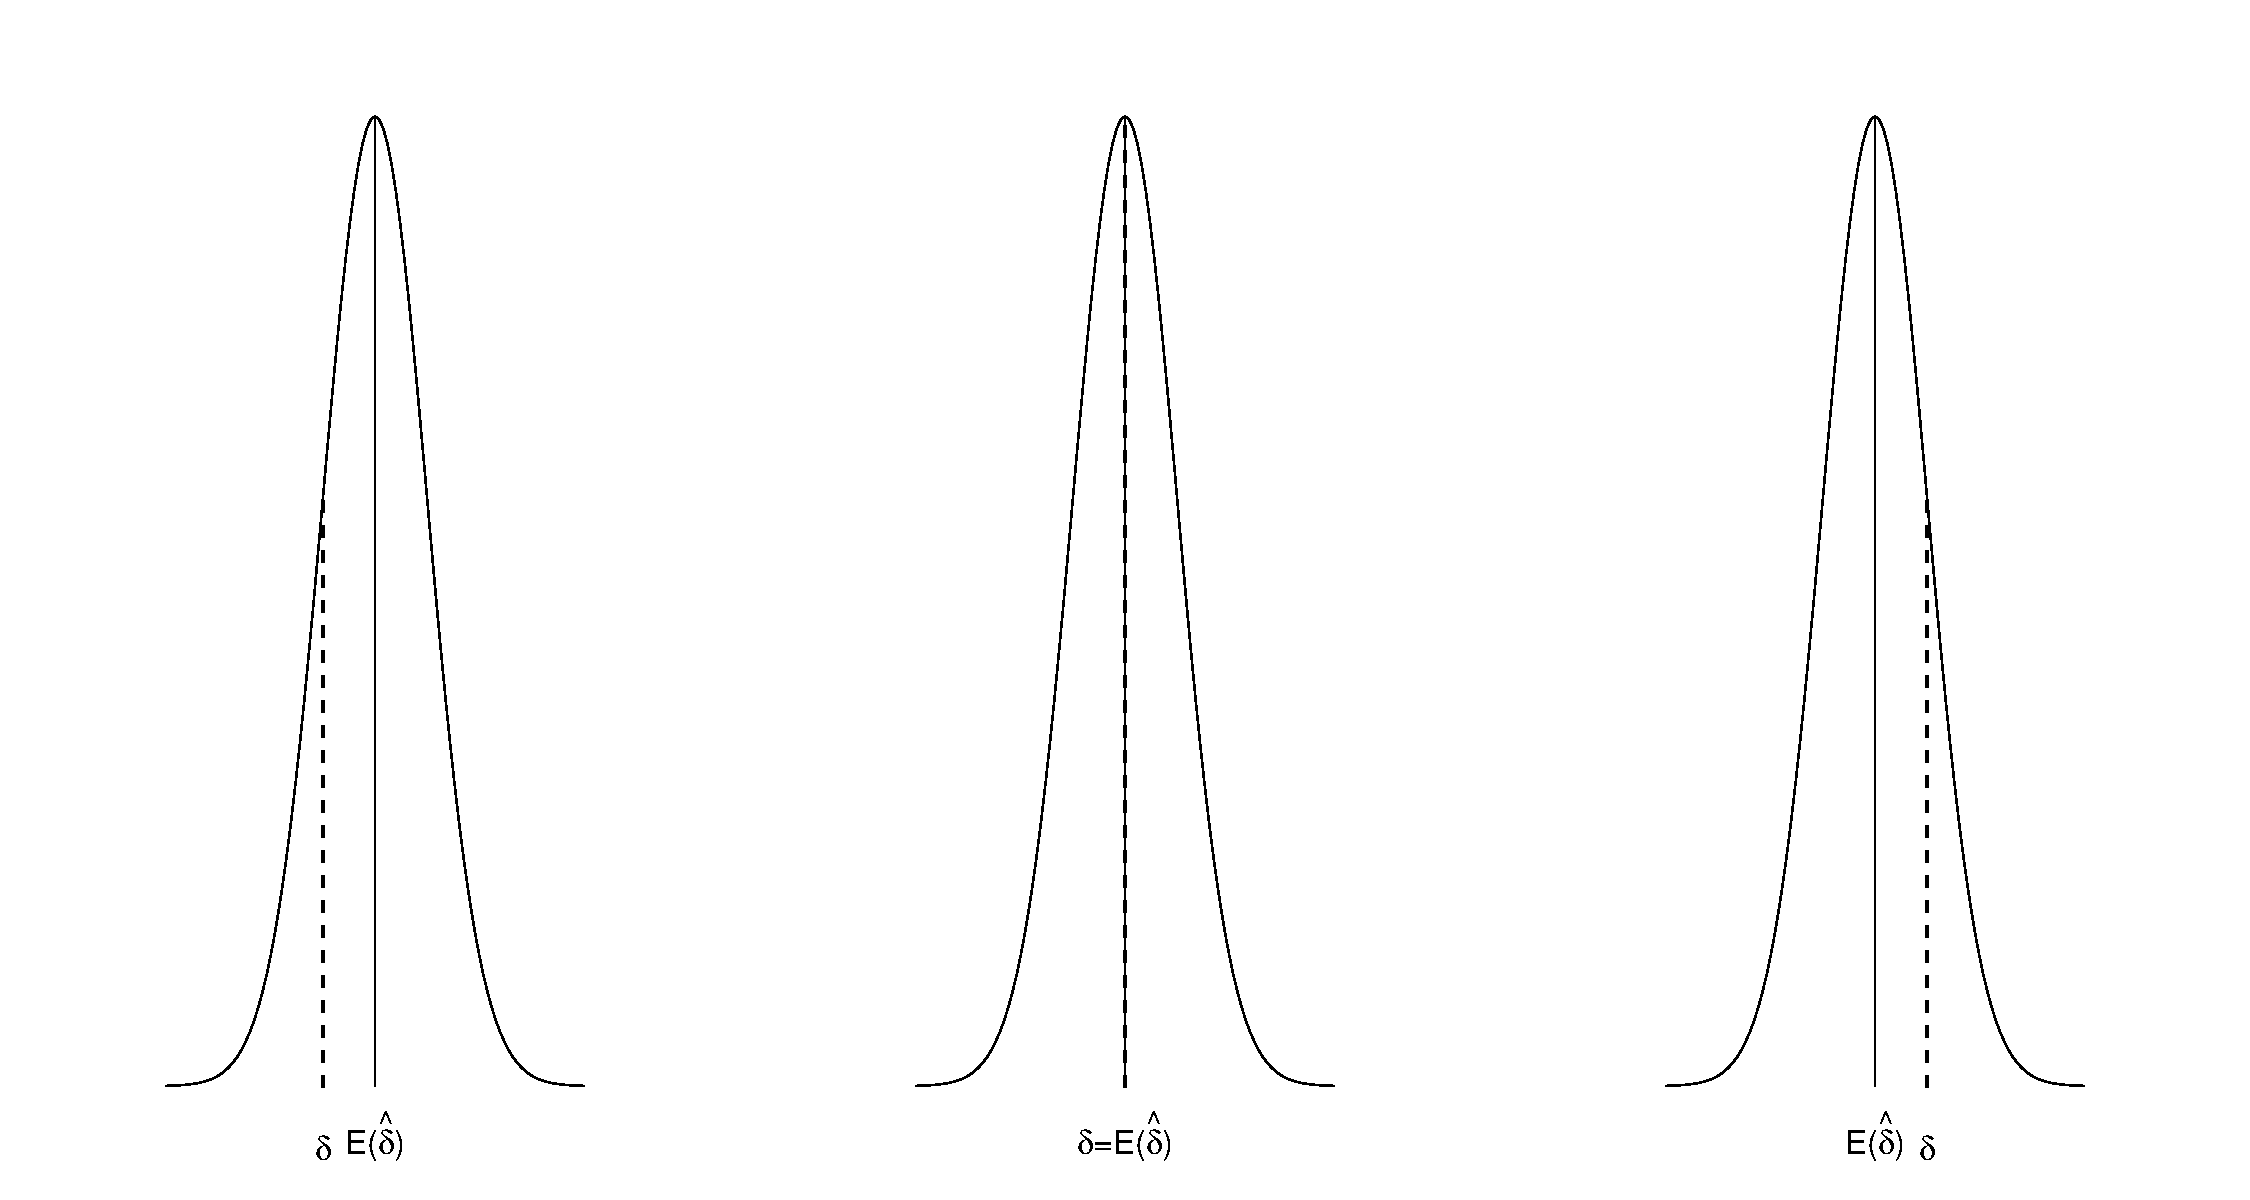
\includegraphics[width=400px]{ES_files/figure-latex/BIAS-1} \caption{Samplig distribution for a positively biased (left), an unbiased (center) and a negatively biased estimator (right)}\label{fig:BIAS}
\end{figure}

Moreover, since there is a strong relationship between the bias and the size of any estimator (the larger an estimator, the larger the bias), it might be interesting to also define the \emph{relative bias} as the ratio between the bias and the population parameter:

\begin{equation} 
\hat{\delta}_{relative \; bias}=\frac{E(\hat{\delta})-\delta}{\delta}
\label{eq:RELBIAS}
\end{equation}

While the bias informs us about the quality of estimates on average, in particular their capacity of lying close to the true value, it says nothing about individual estimates. Imagine a situation where the distribution of estimates is centered around the real parameter but with such a large variance that some point estimates are very far from the center. This would be problematic, since we then do not know if this estimate, based on the sample at hand, is close to the truth or far off. Therefore it is not only essential for an estimator to be unbiased, but the variability of its sampling distribution should also ideally be small. Put simply, we hope that \emph{all} possible estimates are close enough of the true population parameter, in order to be sure that for \emph{any} estimate, one has a correct estimation of the real parameter. Among two unbiased estimators \(\hat{\delta_1}\) and \(\hat{\delta_2}\), we therefore say that \(\hat{\delta_1}\) is \textbf{more efficient} than \(\hat{\delta_2}\) if

\begin{equation} 
Var(\hat{\delta}_1) \leq Var(\hat{\delta}_2)
\label{eq:EFFICIENCY}
\end{equation}

Where \(Var(\hat{\delta})\) is the variance of the sampling distribution of the estimator \(\hat{\delta}\). Among all unbiased estimators, the more efficient will be the one with the smallest variance \footnote{The famous Cramer-Rao inequality provides a theoretical lower bound for the variance of unbiased estimators. An estimator reaching this bound is therefore most efficient.}. Again, the variance of an estimator \(\hat{\delta}\) is a function of its size (the larger the estimator, the larger the variance) and therefore, we might be interested in reducing the effect size impact in computing the \emph{relative variance} as the ratio between the variance and the square of the population estimator:

\begin{equation} 
\hat{\delta}_{relative \; variance}=\frac{Var(\hat{\delta})}{\delta^2}
\label{eq:RELVAR}
\end{equation}

Note that both unbiasedness and efficiency are very important. An unbiased estimator with such a large variance that somes estimates are extremely far from the real parameter is as undesirable as a parameter which is highly biased. In some situations, it is better to have a slightly biased estimator with a tight shape around the biased value (so that each estimate remains relatively close to the true parameter and one can apply bias correction techniques) rather than an unbiased estimator with a large variance (Raviv, 2014).

Finally, the last property of a good point estimator is \textbf{consistency}: consistency means that the bigger the sample size, the closer the estimate is to the population parameter. In other words, the estimates \emph{converge} to the true population parameter.

Beyond the inferential properties, Cumming (2013) reminds that an effect size estimator needs to have a constant value across designs in order to be easily interpretable and to be included in meta-analysis. In other words, it should achieve the property of \textbf{generality}.

\hypertarget{confidence-interval-around-a-point-estimator}{%
\section{Confidence interval around a point estimator}\label{confidence-interval-around-a-point-estimator}}

We already mentioned that confidence interval around a point estimate could replace conventional hypothesis testing. A confidence interval contains all the information that a \(p\)-value of a test based on the same estimator does: if the area of the null hypothesis is out of the \((1-\alpha)\)-confidence interval, then the hypothesis test would also result in a \emph{p}-value below the nominal alpha level. Hypothesis tests and confidence intervals based on the same statistical quantity (this is an essential requirement) are thus directly related. At the same time, the intervals provide extra information about the precision of the sample estimate for inferential purposes, and therefore on how confident we can be in the observed results (Altman, 2005; Ellis, 2015): the narrower the interval, the higher the precision. On the other hand, the wider the confidence interval, the more the data lacks precision (for example, because the sample size is too small).

\hypertarget{different-measures-of-effect-sizes}{%
\section{Different measures of effect sizes}\label{different-measures-of-effect-sizes}}

The \emph{d}-family effect sizes are commonly used with \enquote{between-subject} designs where individuals are randomly assigned into one of two independent groups and groups scores means are compared. The population effect size is defined as

\begin{equation} 
\delta = \frac{\mu_{1}-\mu_{2}}{\sigma} 
\label{eq:Cohendelta}
\end{equation}

where both populations follow a normal distribution with mean \(\mu_j\) in the \(j^{th}\) population (j=1,2) and common standard deviation \(\sigma\). They exist different estimators of this effect size measure. For all of them, the mean difference is estimated by the difference \(\bar{X}_1-\bar{X}_2\) of both sample means. When the equality of variances assumption is assumed, \(\sigma\) is estimated by pooling both samples standard deviations (\(S_1\) and \(S_2\)). When the equality of variances assumption cannot be assumed, alternatives to the common standard deviation are available. Throughout this section, we will present some of these estimators, separately depending on whether they rely on the assumption of equality of variances or not. For each of them, we will provide information about their theoretical bias, variance and consistency.

\hypertarget{when-variances-are-equal-between-groups}{%
\subsection{When variances are equal between groups}\label{when-variances-are-equal-between-groups}}

When we have good reasons to assume equality of variances between groups, then the most common estimator of \(\delta\) is Cohen's \(d_{s}\) where the sample mean difference is divided by a pooled error term (Cohen, 1965):
\begin{equation} 
Cohen's \; d_s = \frac{\bar{X}_1-\bar{X}_2}{\sqrt{\frac{(n_1-1) \times S_1^2+(n_2-1) \times S_2^2}{n_1+n_2-2}}}
\label{eq:Cohends}
\end{equation}

Where \(S_j\) is the standard deviation and \(n_j\) the sample size of the \(j^{th}\) sample (j=1,2). The reasoning behind this measure is to make use of the fact that both samples share the same population variance (Keselman, Algina, Lix, Deering, \& Wilcox, 2008), hence we achieve a more accurate estimation of the population variance by pooling both estimates of this parameter (i.e \(S_1\) and \(S_2\)). Since the larger the sample size, the more accurate the estimate, we give more weight to the estimate based on the larger sample size. Cohen's \(d_{s}\) is directly related with Student's \emph{t}-statistic:

\begin{equation} 
cohen's \; d_s =  t_{student} \times \sqrt{\frac{n_1+n_2}{n_1n_2}}
\label{eq:Cohenvsstudent}
\end{equation}

Under the assumption of normality and equal variances between groups, Student's \emph{t}-statistic follows a \emph{t}-distribution with known degrees of freedom and noncentrality parameter \footnote{Under the null hypothesis of no differences between sample means, Student's $t$-statistic will follow a central $t$-distribution with $n_1+n_2-2$ degrees of freedom. However, when the null hypothesis is false, the distribution of this quantity will not be centered, and noncentral $t$-distribution will arise.}:

\begin{equation} 
df_{student} = n_1+n_2-2
\label{eq:studentdf}
\end{equation}

\begin{equation} 
ncp_{student} = \frac{\mu_1-\mu_2}{\sigma_{pooled}} \times \sqrt{\frac{n_1n_2}{n_1+n_2}}, \;\;\; where \; \sigma_{pooled}= \sqrt{\frac{(n_1-1) \times \sigma^2_1+(n_2-1) \times \sigma^2_2}{n_1+n_2-2}}
\label{eq:studentncp}
\end{equation}

The relationship described in equation \ref{eq:Cohenvsstudent} and the theoretical distribution of Student's \emph{t}-statistic allow us to theoretically determine the sampling distribution of Cohen's \(d_s\), and therefore, its theoretical expectancy and variance when the assumptions of normality and equal variances are met. All these equations are provided in Table 1. For interested readers, bias and variance of Cohen's \(d_s\) have been thoroughly studied, based on Table 1, so as to determine the way different parameters influence them, and results are detailed and available on Github (see Supplemental Material 1 in \url{https://github.com/mdelacre/Effect-sizes/}; it will be the same for all estimators described later).

While Cohen's \(d_s\) is a consistent estimator, its bias and variance are substantial with small sample sizes, even under the assumptions of normality and equal variances (Lakens, 2013). In order to compensate for Cohen's \(d_s\) bias with small sample sizes, Hedges \& Olkin (1985) has defined a bias-corrected version:

\begin{equation} 
Hedges' \; g_s = Cohen's \; d_s \times \frac{\Gamma(\frac{df_{Student}}{2})}{\sqrt{\frac{df_{Student}}{2}} \times \Gamma(\frac{df_{Student}-1}{2})}
\label{eq:Hedgesgs}
\end{equation}

Where \(df_{Student}\) has been defined in equation \ref{eq:studentdf},and \(\Gamma()\) is the gamma function. This equation can be approximated as follows:

\begin{equation} 
Hedges' \; g_s = Cohen's \; d_s \times \left( 1- \frac{3}{4N -9} \right)
\label{eq:Hedgesgsapprox}
\end{equation}

Hedges' \(g_s\) is theoretically unbiased when the assumptions of normality and equal variances are met (see Table 1), and it has a smaller variance than Cohen's \(d_s\), especially with small sample sizes \footnote{$.52 \le \left[\frac{\Gamma(\frac{df}{2})}{\sqrt{\frac{df}{2}} \times \Gamma(\frac{df-1}{2})} \right] ^2 < 1$ for $3 \le df < \infty$. The larger the total sample size, the smaller the difference between the variance of Cohen's $d_s$ and Hedges' $g_s$.}. As Cohen's \(d_s\), its variance depends on the total sample size (N), the sample sizes ratio \(\left( \frac{n_1}{n_2}\right)\) and the population effect size (\(\delta_{Cohen}\)). How these parameters influence the variance of Hedges' \(g_s\) will be summarized in a later section in which we will compare different estimators through Monte Carlo simulations (see the section \enquote{Monte Carlo Simulations}).

While the pooled error term is the best choice when variances are equal between groups (Grissom \& Kim, 2001), it may not be well advised for use with data that violate this assumption (Cumming, 2013; Grissom \& Kim, 2001, 2005; Kelley, 2005, 2005; Shieh, 2013). When variances are unequal between groups, the expression in equation \ref{eq:Cohendelta} is no longer valid because both groups don't share a common population variance. If we pool the estimates of two unequal population variances, the estimator of effect size will be lower as it should be in case of positive pairing (i.e.~the group with the larger sample size is extracted from the population with the larger variance) and larger as it should be in case of negative pairing (i.e.~the group with the larger sample size is extracted from the population with the smaller variance). Because the assumption of equal variances across populations is very rare in practice (Cain, Zhang, \& Yuan, 2017; Delacre et al., 2017; Delacre, Leys, Mora, \& Lakens, 2019; Erceg-Hurn \& Mirosevich, 2008; Glass, Peckham, \& Sanders, 1972; Grissom, 2000; Micceri, 1989; Yuan, Bentler, \& Chan, 2004), both Cohen's \(d_s\) and Hedges' \(g_s\) should be abandoned in favor of an alternative robust to unequal population variances.

\newpage
\begin{landscape}

\begin{longtable}[]{@{}lccc@{}}
\caption{Expentency, bias and variance of Cohen's \(d_s\) and Hedges' \(g_s\) under the assumptions that independent residuals are normally distributed with equal variances across groups.}\tabularnewline
\toprule
\begin{minipage}[b]{0.12\columnwidth}\raggedright
\strut
\end{minipage} & \begin{minipage}[b]{0.11\columnwidth}\centering
df\strut
\end{minipage} & \begin{minipage}[b]{0.24\columnwidth}\centering
Expectancy\strut
\end{minipage} & \begin{minipage}[b]{0.42\columnwidth}\centering
Variance\strut
\end{minipage}\tabularnewline
\midrule
\endfirsthead
\toprule
\begin{minipage}[b]{0.12\columnwidth}\raggedright
\strut
\end{minipage} & \begin{minipage}[b]{0.11\columnwidth}\centering
df\strut
\end{minipage} & \begin{minipage}[b]{0.24\columnwidth}\centering
Expectancy\strut
\end{minipage} & \begin{minipage}[b]{0.42\columnwidth}\centering
Variance\strut
\end{minipage}\tabularnewline
\midrule
\endhead
\begin{minipage}[t]{0.12\columnwidth}\raggedright
\(Cohen's \; d_s\)\strut
\end{minipage} & \begin{minipage}[t]{0.11\columnwidth}\centering
\(N-2\)\strut
\end{minipage} & \begin{minipage}[t]{0.24\columnwidth}\centering
\(\delta_{cohen} \times \frac{\sqrt{\frac{df}{2}} \times \Gamma(\frac{df-1}{2})}{\Gamma(\frac{df}{2})}\)\strut
\end{minipage} & \begin{minipage}[t]{0.42\columnwidth}\centering
\(\frac{N\times df}{n_1n_2 \times (df-2)} + \delta^2_{Cohen} \left[ \frac{df}{df-2} - \left( \frac{\sqrt{\frac{df}{2}} \times \Gamma \left(\frac{df-1}{2} \right)}{\Gamma \left( \frac{df}{2}\right)}\right)^2\right]\)\strut
\end{minipage}\tabularnewline
\begin{minipage}[t]{0.12\columnwidth}\raggedright
\strut
\end{minipage} & \begin{minipage}[t]{0.11\columnwidth}\centering
\strut
\end{minipage} & \begin{minipage}[t]{0.24\columnwidth}\centering
\strut
\end{minipage} & \begin{minipage}[t]{0.42\columnwidth}\centering
\strut
\end{minipage}\tabularnewline
\begin{minipage}[t]{0.12\columnwidth}\raggedright
\strut
\end{minipage} & \begin{minipage}[t]{0.11\columnwidth}\centering
\strut
\end{minipage} & \begin{minipage}[t]{0.24\columnwidth}\centering
\(\approx \frac{\delta_{Cohen}}{\left(1-\frac{3}{4N-9}\right)}\)\strut
\end{minipage} & \begin{minipage}[t]{0.42\columnwidth}\centering
\(\approx \frac{N\times df}{n_1n_2 \times (df-2)} + \delta^2_{Cohen} \left[ \frac{df}{df-2} - \left( \frac{1}{1-\frac{3}{4N-9} }\right)^2\right]\)\strut
\end{minipage}\tabularnewline
\begin{minipage}[t]{0.12\columnwidth}\raggedright
\strut
\end{minipage} & \begin{minipage}[t]{0.11\columnwidth}\centering
\strut
\end{minipage} & \begin{minipage}[t]{0.24\columnwidth}\centering
\strut
\end{minipage} & \begin{minipage}[t]{0.42\columnwidth}\centering
\strut
\end{minipage}\tabularnewline
\begin{minipage}[t]{0.12\columnwidth}\raggedright
\strut
\end{minipage} & \begin{minipage}[t]{0.11\columnwidth}\centering
\strut
\end{minipage} & \begin{minipage}[t]{0.24\columnwidth}\centering
\strut
\end{minipage} & \begin{minipage}[t]{0.42\columnwidth}\centering
\strut
\end{minipage}\tabularnewline
\begin{minipage}[t]{0.12\columnwidth}\raggedright
\(Hedges's \; g_s\)\strut
\end{minipage} & \begin{minipage}[t]{0.11\columnwidth}\centering
\(N-2\)\strut
\end{minipage} & \begin{minipage}[t]{0.24\columnwidth}\centering
\(\delta_{Cohen}\)\strut
\end{minipage} & \begin{minipage}[t]{0.42\columnwidth}\centering
\(Var(Cohen's \; d_s) \times \left[ \frac{\Gamma(\frac{df}{2})}{\sqrt{\frac{df}{2}} \times \Gamma(\frac{df-1}{2})} \right]^2\)\strut
\end{minipage}\tabularnewline
\begin{minipage}[t]{0.12\columnwidth}\raggedright
\strut
\end{minipage} & \begin{minipage}[t]{0.11\columnwidth}\centering
\strut
\end{minipage} & \begin{minipage}[t]{0.24\columnwidth}\centering
\strut
\end{minipage} & \begin{minipage}[t]{0.42\columnwidth}\centering
\strut
\end{minipage}\tabularnewline
\begin{minipage}[t]{0.12\columnwidth}\raggedright
\strut
\end{minipage} & \begin{minipage}[t]{0.11\columnwidth}\centering
\strut
\end{minipage} & \begin{minipage}[t]{0.24\columnwidth}\centering
\strut
\end{minipage} & \begin{minipage}[t]{0.42\columnwidth}\centering
\(\approx Var(Cohen's \; d_s) \times \left[1-\frac{3}{4N-9}\right]^2\)\strut
\end{minipage}\tabularnewline
\begin{minipage}[t]{0.12\columnwidth}\raggedright
\strut
\end{minipage} & \begin{minipage}[t]{0.11\columnwidth}\centering
\strut
\end{minipage} & \begin{minipage}[t]{0.24\columnwidth}\centering
\strut
\end{minipage} & \begin{minipage}[t]{0.42\columnwidth}\centering
\strut
\end{minipage}\tabularnewline
\bottomrule
\end{longtable}

\emph{Note}. Cohen's \(d_s\) is a biased estimator, because its expectation differ from the population effect size. On the other hand, Hedges' \(g_s\) is an unbiased estimator, because its expectation equals the population effect size; equations in Table 1 require \(df \ge 3\) (i.e.~\(N \ge 5\)).

\end{landscape}

\hypertarget{when-variances-are-unequal-between-populations}{%
\subsection{When variances are unequal between populations}\label{when-variances-are-unequal-between-populations}}

In his review, Shieh (2013) mentions three options available in the literature to deal with the case of unequal variances: the sample mean difference divided by (A) the Glass's \(d_s\), (B) the Shieh's \(d_s\) and (C) the non pooled average of both variance estimates.

\hypertarget{glasss-d_s}{%
\subsubsection{\texorpdfstring{Glass's \(d_s\)}{Glass's d\_s}}\label{glasss-d_s}}

When comparing one control group with one experimental group, Glass, McGav, \& Smith (2005) recommend using the standard deviation \(SD\) of the control group as standardizer. It is also advocated by Cumming (2013), because, according to him, it is what makes the most sense, conceptually speaking. This yields

\begin{equation} 
Glass's \; d_s = \frac{\bar{X}_{e} - \bar{X}_{c}}{S_{c}}
\label{eq:Glassds}
\end{equation}

Where \(\bar{X}_{e} \; and \; \bar{X}_{c}\) are respectively the sample means of the experimental and control groups, and \(S_{c}\) is the sample SD of the control group. One argument in favour of using the \(SD\) of the control group as standardizer is the fact that it is not affected by the experimental treatment. When it is easy to identify which group is the \enquote{control} one, it is therefore convenient to compare the effect size estimation of different designs studying the same effect. However, defining this group is not always obvious (Coe, 2002). This could induce large ambiguity because depending of the chosen \(SD\) as standardizer, measures could be substantially different (Shieh, 2013).

The distribution of Glass's \(d_{s}\) is defined as following (Algina, Keselman, \& Penfield, 2006):

\begin{equation} 
Glass's \; d_s \sim \sqrt{\frac{1}{n_{c}}+\frac{S_{e}^2}{n_{e} \times S^2_{c}}} \times t_{df,ncp}
\label{eq:glassvst}
\end{equation}

Where \(n_c\) and \(n_e\) are respectively the sample sizes of the control and experimental groups, and \(df\) and \(ncp\) are defined as follows:

\begin{equation} 
df = n_{c}-1
\label{eq:glassdf}
\end{equation}

\begin{equation} 
ncp = \frac{\mu_{c}-\mu_{e}}{\sigma_{c} \times \sqrt{\frac{1}{n_{c}} + \frac{\sigma_{e}^2}{n_{e} \times \sigma^2_{c}}}}
\label{eq:glassdf}
\end{equation}

Where \(\mu_c\) and \(\mu_e\) are respectively the mean of the populations control and experimental groups are extracted from. Thanks to equation \ref{eq:glassvst}, we can compute its theoretical expectancy variance when the assumptions of normality is met (See Table 2), and therefore determine which factors influence bias and variance, and how they do so (see Supplemental Material 1).

\newpage
\begin{landscape}

\begin{longtable}[]{@{}lccc@{}}
\caption{Expentency, bias and variance of Glass's \(d_s\) and Cohen's \(d'_s\) and Shieh's \(d_s\) under the assumptions that independent residuals are normally distributed.}\tabularnewline
\toprule
\begin{minipage}[b]{0.10\columnwidth}\raggedright
\strut
\end{minipage} & \begin{minipage}[b]{0.18\columnwidth}\centering
df\strut
\end{minipage} & \begin{minipage}[b]{0.16\columnwidth}\centering
Expectancy\strut
\end{minipage} & \begin{minipage}[b]{0.45\columnwidth}\centering
Variance\strut
\end{minipage}\tabularnewline
\midrule
\endfirsthead
\toprule
\begin{minipage}[b]{0.10\columnwidth}\raggedright
\strut
\end{minipage} & \begin{minipage}[b]{0.18\columnwidth}\centering
df\strut
\end{minipage} & \begin{minipage}[b]{0.16\columnwidth}\centering
Expectancy\strut
\end{minipage} & \begin{minipage}[b]{0.45\columnwidth}\centering
Variance\strut
\end{minipage}\tabularnewline
\midrule
\endhead
\begin{minipage}[t]{0.10\columnwidth}\raggedright
\(Glass's \; d_s\)\strut
\end{minipage} & \begin{minipage}[t]{0.18\columnwidth}\centering
\(n_c-1\)\strut
\end{minipage} & \begin{minipage}[t]{0.16\columnwidth}\centering
~\(\delta_{glass} \times c_f\)\strut
\end{minipage} & \begin{minipage}[t]{0.45\columnwidth}\centering
\(\frac{df}{df-2} \times \left( \frac{1}{n_c} + \frac{\sigma^2_e}{n_e\sigma^2_c}\right) + \delta^2_{Glass} \left( \frac{df}{df-2} - c_f^2 \right)\)\strut
\end{minipage}\tabularnewline
\begin{minipage}[t]{0.10\columnwidth}\raggedright
\strut
\end{minipage} & \begin{minipage}[t]{0.18\columnwidth}\centering
\strut
\end{minipage} & \begin{minipage}[t]{0.16\columnwidth}\centering
\strut
\end{minipage} & \begin{minipage}[t]{0.45\columnwidth}\centering
\strut
\end{minipage}\tabularnewline
\begin{minipage}[t]{0.10\columnwidth}\raggedright
\(Cohen's \; d'_s\)\strut
\end{minipage} & \begin{minipage}[t]{0.18\columnwidth}\centering
\(\frac{(n_1-1)(n_2-1)(s^2_1+s^2_2)^2}{(n_2-1)s^4_1+(n_1-1)s^4_2}\)\strut
\end{minipage} & \begin{minipage}[t]{0.16\columnwidth}\centering
\(\delta'_{Cohen} \times c_f\)\strut
\end{minipage} & \begin{minipage}[t]{0.45\columnwidth}\centering
\(\frac{df}{df-2} \times \frac{2\left( \frac{\sigma^2_1}{n_1} + \frac{\sigma^2_2}{n_2} \right)}{\sigma^2_1+\sigma^2_2} + (\delta'_{Cohen})^2 \left( \frac{df}{df-2} - c_f^2 \right)\)\strut
\end{minipage}\tabularnewline
\begin{minipage}[t]{0.10\columnwidth}\raggedright
\strut
\end{minipage} & \begin{minipage}[t]{0.18\columnwidth}\centering
\strut
\end{minipage} & \begin{minipage}[t]{0.16\columnwidth}\centering
\strut
\end{minipage} & \begin{minipage}[t]{0.45\columnwidth}\centering
\strut
\end{minipage}\tabularnewline
\begin{minipage}[t]{0.10\columnwidth}\raggedright
\strut
\end{minipage} & \begin{minipage}[t]{0.18\columnwidth}\centering
\strut
\end{minipage} & \begin{minipage}[t]{0.16\columnwidth}\centering
\(\approx \delta'_{Cohen} \times \frac{4df-1}{4(df-1)}\)\strut
\end{minipage} & \begin{minipage}[t]{0.45\columnwidth}\centering
\(\approx \frac{df}{df-2} \times \frac{2\left( \frac{\sigma^2_1}{n_1} + \frac{\sigma^2_2}{n_2} \right)}{\sigma^2_1+\sigma^2_2} + (\delta'_{Cohen})^2 \left[ \frac{df}{df-2} - \left( \frac{4 \;df-1}{4(df-1)}\right)^2 \right]\)\strut
\end{minipage}\tabularnewline
\begin{minipage}[t]{0.10\columnwidth}\raggedright
\strut
\end{minipage} & \begin{minipage}[t]{0.18\columnwidth}\centering
\strut
\end{minipage} & \begin{minipage}[t]{0.16\columnwidth}\centering
\strut
\end{minipage} & \begin{minipage}[t]{0.45\columnwidth}\centering
\strut
\end{minipage}\tabularnewline
\begin{minipage}[t]{0.10\columnwidth}\raggedright
\(Shieh's \; d_s\)\strut
\end{minipage} & \begin{minipage}[t]{0.18\columnwidth}\centering
\(\approx \frac{\left(\frac{\sigma^2_1}{n_1}+\frac{\sigma^2_2}{n_2} \right)^2}{\frac{(\sigma^2_1/n_1)^2}{n_1-1}+\frac{(\sigma^2_2/n_2)^2}{n_2-1}}\)\strut
\end{minipage} & \begin{minipage}[t]{0.16\columnwidth}\centering
\(\delta_{Shieh} \times c_f\)\strut
\end{minipage} & \begin{minipage}[t]{0.45\columnwidth}\centering
\(\frac{df}{(df-2)N} + \delta^2_{Shieh} \left( \frac{df}{df-2} - c_f^2 \right)\)\strut
\end{minipage}\tabularnewline
\begin{minipage}[t]{0.10\columnwidth}\raggedright
\strut
\end{minipage} & \begin{minipage}[t]{0.18\columnwidth}\centering
\strut
\end{minipage} & \begin{minipage}[t]{0.16\columnwidth}\centering
\strut
\end{minipage} & \begin{minipage}[t]{0.45\columnwidth}\centering
\strut
\end{minipage}\tabularnewline
\bottomrule
\end{longtable}

\emph{Note}. \(c_f=\frac{\sqrt{\frac{df}{2}} \times \Gamma\left( \frac{df-1}{2}\right)}{\Gamma\left( \frac{df}{2}\right)}\); all estimators are biased estimators, because their expectations differ from the population effect size \(\delta\); equations require \(df \ge 3\) and at least 2 subjects per group.

\end{landscape}
\newpage

\hypertarget{shiehs-d_s}{%
\subsubsection{\texorpdfstring{Shieh's \(d_s\)}{Shieh's d\_s}}\label{shiehs-d_s}}

Kulinskaya \& Staudte (2007) were the first to advice the use of a standardizer that takes the sample sizes allocation ratios into account, in addition to the variance of both samples. Shieh (2013), following Kulinskaya \& Staudte (2007), proposed a modification of the exact \emph{SD} of the sample mean difference:

\begin{equation} 
Shieh's \; d_s = \frac{\bar{X}_1 - \bar{X}_2}{\sqrt{S_1^2/q_1+S_2^2/q_2}}; \;\;\; q_j=\frac{n_j}{N} (j=1,2)
\label{eq:Shiehds}
\end{equation}

where \(N = n_1+n_2\). Shieh's \(d_{s}\) is directly related with Welch's \emph{t}-statistic:

\begin{equation} 
t_{welch} = Shieh's \; d_s \times \sqrt{N}
\label{eq:shiehvswelch}
\end{equation}

Where \(N = n_1+n_2\). The exact distribution of Welch's \emph{t}-statistic is more complicated than the exact distribution of Student's \emph{t}-statistic, but it follows a \emph{t}-distribution with degrees of freedom and noncentrality parameters that can be approximated as follows, under the assumption of normality (Shieh, 2013; Welch, 1938):

\begin{equation} 
df_{Welch} \approx \frac{\left(\frac{\sigma^2_1}{n_1}+\frac{\sigma^2_2}{n_2} \right)^2}{\frac{(\sigma^2_1/n_1)^2}{n_1-1}+\frac{(\sigma^2_2/n_2)^2}{n_2-1}}
\label{eq:welchdf}
\end{equation}

\begin{equation} 
ncp_{Welch} = \frac{\mu_1-\mu_2}{\sqrt{\frac{\sigma_1^2}{n_1/N}+\frac{\sigma_2^2}{n_2/N}}} \times \sqrt{N}
\label{eq:welchncp}
\end{equation}

The relationship described in equation \ref{eq:shiehvswelch} and the theoretical distribution of Welch's \emph{t}-statistic allow us to theoretically approximate the sampling distribution of Shieh's \(d_s\). Based on the sampling distribution of Shieh's \(d_s\), we can estimate its theoretical expectancy and variance under the assumption of normality (see Table 2), and therefore determine which factors influence bias and variance, and how they do so (see Supplemental Material 1).

It can be demonstrated that when variances and sample sizes are equal across groups, the biases and variances of Shieh's \(d_s\) and Cohen's \(d_s\) are identical except for a constant, as shown in equations \ref{eq:biascohenshieh} and \ref{eq:varcohenshieh}:

\begin{equation} 
Shieh's \; d_{s,bias} = 2 \times Cohen's \; d_{s,bias} \;\;\;(considering \; \sigma_1 = \sigma_2 \; and \; n_1 = n_2)
\label{eq:biascohenshieh}
\end{equation}

\begin{equation} 
Shieh's \; d_{s,variance} = 4 \times Cohen's \; d_{s,variance} \;\;\;(considering \; \sigma_1 = \sigma_2 \; and \; n_1 = n_2)
\label{eq:varcohenshieh}
\end{equation}

Due to the relation described in equation \ref{eq:cohenshieh} when sample sizes are equal between groups (as explained in Supplemental Material 2), such proportions mean that relative to their respective true effect size, Cohen's \(d_s\) and Shieh's \(d_s\) are equally good. This is a good illustration of the fact that biases and variances should always be studied relative to the population effect size (and not in absolute terms), as we will do later.

\begin{equation} 
Shieh's \; \delta_{n_1=n_2}= \frac{Cohen's \; \delta_{n_1=n_2}}{2}
\label{eq:cohenshieh}
\end{equation}

Except for this very specific situation, according to the statistical properties of Welch's statistic under heteroscedasticity, Shieh's \(d_s\) accounts for the sample sizes allocation ratio. The lack of generality caused by taking this specificity of the design into account has led Cumming (2013) to question its usefulness in terms of interpretability: when keeping constant the mean difference (\(\bar{X_1}-\bar{X_2}\)) as well as \(SD_1\) and \(SD_2\), Shieh's \(d_s\) will vary as a function of the sample sizes allocation ratio (the dependency of Shieh's \(d_s\) value on the sample sizes allocation ratio is illustrated in the following shiny application: \url{https://mdelacre.shinyapps.io/ShiehvsCohen/}).

\hypertarget{cohens-d_s}{%
\subsubsection{\texorpdfstring{Cohen's \(d'_s\)}{Cohen's d'\_s}}\label{cohens-d_s}}

The sample mean difference, divided by the non pooled average of both variance estimates was suggested by Welch (1938). This yields:

\begin{equation} 
Cohen's \; d'_s = \frac{\bar{X}_{1} - \bar{X}_{2}}{ \sqrt{\frac{\left(S^2_{1}+S^2_{2} \right)}{2}}}
\label{eq:cohenprimeds}
\end{equation}

Where \(\bar{X}_{j}\) is the mean and \(S_j\) is the standard deviation of the \(j^{th}\) sample (j = 1,2). We know the distribution of Cohen's \(d'_{s}\) (Huynh, 1989):

\begin{equation} 
cohen's \; d'_s \sim  \sqrt{\frac{\left( \frac{\sigma^2_1}{n_1}+\frac{\sigma^2_2}{n_2}\right)(\sigma^2_1+\sigma^2_2)}{2}} \times t_{df^*,ncp^*}
\label{eq:cohendprimedist}
\end{equation}

Where \(df^*\) and \(ncp^*\) are defined as follows:

\begin{equation} 
df^* = \frac{(n_1-1)(n_2-1)(s^2_1+s^2_2)^2}{(n_2-1)s^4_1+(n_1-1)s^4_2}
\label{eq:cohendprimedf}
\end{equation}

\begin{equation} 
ncp^*=\frac{\mu_1-\mu_2}{\sqrt{\frac{\sigma^2_1+\sigma^2_2}{2}}} \times \sqrt{\frac{n_1n_2(\sigma^2_1+\sigma^2_2)}{2(n_2\sigma^2_1+n_1\sigma^2_2)}}
\label{eq:cohendprimevst}
\end{equation}

Thanks to equation \ref{eq:cohendprimevst}, we can compute its theoretical expectancy variance when the assumptions of normality is met (See Table 2), and therefore determine which factors influence bias and variance, and how they do so (see Supplemental Material 1). This estimator has been widely criticized, because:\\
- it results in a variance term of an artificial population and is therefore very difficult to interpret (Grissom \& Kim, 2001);\\
- unless both sample sizes are equal, the variance term does not correspond to the variance of the mean difference (Shieh, 2013).

However, we will show throughout the simulation section that this estimator show very good inferential properties.

\hypertarget{glasss-g_s-shiehs-g_s-and-hedges-g_s}{%
\subsubsection{\texorpdfstring{Glass's \(g_s\), Shieh's \(g_s\) and Hedges' \(g'_s\)}{Glass's g\_s, Shieh's g\_s and Hedges' g'\_s}}\label{glasss-g_s-shiehs-g_s-and-hedges-g_s}}

As for Cohen's \(d_s\), an Hedges' correction can be applied in order to compensate for the bias of Glass's \(d_s\), Shieh's \(d_s\) and Cohen's \(d'_s\) with small sample sizes (see Table 2). This correction has the following general form:

\begin{equation} 
g_s = d_s \times \frac{\Gamma(\frac{\nu}{2})}{\sqrt{\frac{\nu}{2}} \times \Gamma(\frac{\nu-1}{2})}
\label{eq:Hedgesgs}
\end{equation}

Where \(\nu\) are provided in equation \ref{eq:glassdf} for Glass's \(g_s\), in equation \ref{eq:cohendprimedf} for Hedges' \(g'_s\) and in equation \ref{eq:welchdf} for Shieh's \(g_s\). The three corrected estimators are theoretically unbiased when the assumptions of normality is met. Their variance are a function of the same factors as their biased equivalent, however, due to the correction, they have a smaller variance, especially with small sample size, as shown in Table 3. In summary:

\begin{itemize}
\tightlist
\item
  The variances of Hedges' \(g'_s\) and Shieh's \(g_s\) depend on the total sample size (\(N\)), their respective population effect size (\(\delta\)), and the interaction between the sample sizes ratio and the \(SD\)-ratio \(\left(\frac{n_1}{n_2}\times\frac{\sigma_1}{\sigma_2} \right)\).\\
\item
  The variance of Glass's \(g_s\) also depends on \(N\), \(\delta\) and \(\frac{n_1}{n_2}\times\frac{\sigma_1}{\sigma_2}\). In addition, there is also a main effect of the \(SD\)-ratio \(\left(\frac{\sigma_1}{\sigma_2} \right)\) on its variance.
\end{itemize}

How these parameters influence the variance of the estimators will be summarized and illustrated in the section dedicated to the Monte Carlo simulations.

\newpage
\begin{landscape}

\begin{longtable}[]{@{}lccc@{}}
\caption{Expentency, bias and variance of Glass's \(d_s\) and Cohen's \(d'_s\) and Shieh's \(d_s\) under the assumptions that independent residuals are normally distributed.}\tabularnewline
\toprule
\begin{minipage}[b]{0.10\columnwidth}\raggedright
\strut
\end{minipage} & \begin{minipage}[b]{0.18\columnwidth}\centering
df\strut
\end{minipage} & \begin{minipage}[b]{0.16\columnwidth}\centering
Expectancy\strut
\end{minipage} & \begin{minipage}[b]{0.45\columnwidth}\centering
Variance\strut
\end{minipage}\tabularnewline
\midrule
\endfirsthead
\toprule
\begin{minipage}[b]{0.10\columnwidth}\raggedright
\strut
\end{minipage} & \begin{minipage}[b]{0.18\columnwidth}\centering
df\strut
\end{minipage} & \begin{minipage}[b]{0.16\columnwidth}\centering
Expectancy\strut
\end{minipage} & \begin{minipage}[b]{0.45\columnwidth}\centering
Variance\strut
\end{minipage}\tabularnewline
\midrule
\endhead
\begin{minipage}[t]{0.10\columnwidth}\raggedright
\(Glass's \; g_s\)\strut
\end{minipage} & \begin{minipage}[t]{0.18\columnwidth}\centering
\(n_c-1\)\strut
\end{minipage} & \begin{minipage}[t]{0.16\columnwidth}\centering
~\(\delta_{glass}\)\strut
\end{minipage} & \begin{minipage}[t]{0.45\columnwidth}\centering
\(Var(Glass's \; d_s) \times \left( \frac{\Gamma\left(\frac{df}{2} \right)}{\sqrt{\frac{df}{2}} \times \Gamma \left( \frac{df-1}{2}\right)}\right)^2\)\strut
\end{minipage}\tabularnewline
\begin{minipage}[t]{0.10\columnwidth}\raggedright
\strut
\end{minipage} & \begin{minipage}[t]{0.18\columnwidth}\centering
\strut
\end{minipage} & \begin{minipage}[t]{0.16\columnwidth}\centering
\strut
\end{minipage} & \begin{minipage}[t]{0.45\columnwidth}\centering
\strut
\end{minipage}\tabularnewline
\begin{minipage}[t]{0.10\columnwidth}\raggedright
\(Cohen's \; g'_s\)\strut
\end{minipage} & \begin{minipage}[t]{0.18\columnwidth}\centering
\(\frac{(n_1-1)(n_2-1)(s^2_1+s^2_2)^2}{(n_2-1)s^4_1+(n_1-1)s^4_2}\)\strut
\end{minipage} & \begin{minipage}[t]{0.16\columnwidth}\centering
\(\delta'_{Cohen}\)\strut
\end{minipage} & \begin{minipage}[t]{0.45\columnwidth}\centering
\(Var(Cohen's \; d'_s) \times \left( \frac{\Gamma\left(\frac{df}{2} \right)}{\sqrt{\frac{df}{2}} \times \Gamma \left( \frac{df-1}{2}\right)}\right)^2\)\strut
\end{minipage}\tabularnewline
\begin{minipage}[t]{0.10\columnwidth}\raggedright
\strut
\end{minipage} & \begin{minipage}[t]{0.18\columnwidth}\centering
\strut
\end{minipage} & \begin{minipage}[t]{0.16\columnwidth}\centering
\strut
\end{minipage} & \begin{minipage}[t]{0.45\columnwidth}\centering
\strut
\end{minipage}\tabularnewline
\begin{minipage}[t]{0.10\columnwidth}\raggedright
\(Shieh's \; g_s\)\strut
\end{minipage} & \begin{minipage}[t]{0.18\columnwidth}\centering
\(\approx \frac{\left(\frac{\sigma^2_1}{n_1}+\frac{\sigma^2_2}{n_2} \right)^2}{\frac{(\sigma^2_1/n_1)^2}{n_1-1}+\frac{(\sigma^2_2/n_2)^2}{n_2-1}}\)\strut
\end{minipage} & \begin{minipage}[t]{0.16\columnwidth}\centering
\(\delta_{Shieh}\)\strut
\end{minipage} & \begin{minipage}[t]{0.45\columnwidth}\centering
\(Var(Shieh's \; d_s) \times \left( \frac{\Gamma\left(\frac{df}{2} \right)}{\sqrt{\frac{df}{2}} \times \Gamma \left( \frac{df-1}{2}\right)}\right)^2\)\strut
\end{minipage}\tabularnewline
\begin{minipage}[t]{0.10\columnwidth}\raggedright
\strut
\end{minipage} & \begin{minipage}[t]{0.18\columnwidth}\centering
\strut
\end{minipage} & \begin{minipage}[t]{0.16\columnwidth}\centering
\strut
\end{minipage} & \begin{minipage}[t]{0.45\columnwidth}\centering
\strut
\end{minipage}\tabularnewline
\bottomrule
\end{longtable}

\emph{Note}. \(c_f=\frac{\sqrt{\frac{df}{2}} \times \Gamma\left( \frac{df-1}{2}\right)}{\Gamma\left( \frac{df}{2}\right)}\); all estimators are unbiased estimators, because their expectations equal the population effect size \(\delta\); equations require \(df \ge 3\) and at least 2 subjects per group.

\end{landscape}
\newpage

\hypertarget{monte-carlo-simulations-assessing-the-bias-efficiency-and-consistency-of-5-estimators}{%
\subsection{Monte Carlo Simulations: assessing the bias, efficiency and consistency of 5 estimators}\label{monte-carlo-simulations-assessing-the-bias-efficiency-and-consistency-of-5-estimators}}

\hypertarget{method}{%
\paragraph{Method}\label{method}}

We performed Monte Carlo simulations using R (version 3.5.0) to assess the bias, efficiency and consistency of Cohen's \(g_s\), Glass's \(g_s\) (using respectively the sample \(SD\) of the first or second group as a standardizer), Hedges' \(g'_s\) and Shieh's \(g_s\).

A set of 100,000 datasets were generated for 1,008 scenarios as a function of different criterions that will be explained below. In 252 scenarios, samples were extracted from a normally distributed population (in order to insure the reliability of our calculation method) and in 756 scenarios, samples were extracted from non normal population distributions. In order to assess the quality of estimators under realistic deviations from the normality assumption, we referred to the review of Cain et al. (2017). Cain et al.~(2017) investigated 1,567 univariate distributions from 194 studies published by authors in Psychological Science (from January 2013 to June 2014) and the American Education Research Journal (from January 2010 to June 2014). For each distribution, they computed the Fisher's skewness (G1) and kurtosis (G2):
\begin{equation} 
G_{1}=\frac{\sqrt{n(n-1)}}{n-2} \frac{m_{3}}{\sqrt{(m_{2})^3}}
\label{eq:skew}
\end{equation}

with n = sample size, \(m_{2}\) = second centered moment and \(m_{3}\) = third centered moment.

\begin{equation} 
G_{2}=\frac{n-1}{(n-2)(n-3)}\times [(n+1)(\frac{m_{4}}{(m_{2})^2}-3)+6]
\label{eq:kurt}
\end{equation}

with n = sample size and \(m_{2}\) and \(m_{4}\) = the second and fourth centered moments. They found values of kurtosis from G2 = -2.20 to 1,093.48. According to their suggestions, throughout our simulations, we kept constant the population kurtosis value at the 99th percentile of their distribution of kurtosis, i.e.~G2=95.75. Regarding skewness, we simulated population parameter values which correspond to the 1st and 99th percentile of their distribution of skewness, i.e.~respectively G1 = -2.08 and G1 = 6.32. We also simulated samples extracted from population where G1 = 0, in order to assess the main effect of high kurtosis on the quality of estimators. All possible combinations of population skewness and kurtosis and the number of scenarios for each combination are summarized in Table 4.

\newpage

\begin{longtable}[]{@{}ccccc@{}}
\caption{Number of Combinations of skewness and kurtosis in our simulations.}\tabularnewline
\toprule
& & & \textbf{Kurtosis} &\tabularnewline
\midrule
\endfirsthead
\toprule
& & & \textbf{Kurtosis} &\tabularnewline
\midrule
\endhead
& & 0 & 95.75 & \textbf{TOTAL}\tabularnewline
& & --------------- & -------------- & ---------------\tabularnewline
& 0 & 252 & 252 & \textbf{504}\tabularnewline
& & & &\tabularnewline
\textbf{Skewness} & -2.08 & / & 252 & \textbf{252}\tabularnewline
& & & &\tabularnewline
& 6.32 & / & 252 & \textbf{252}\tabularnewline
& & & &\tabularnewline
& \textbf{TOTAL} & \textbf{252} & \textbf{756} & \textbf{1008}\tabularnewline
\bottomrule
\end{longtable}

\emph{Note.} Fisher's skewness (G1) and kurtosis (G2) are presented in Table 4. The 252 combinations where both G1 and G2 equal 0 correspond to the normal case.

For the 4 resulting combinations of skewness and kurtosis (see Table 4), all other parameter values were chosen in order to illustrate the consequences of factors identified as playing a key role on the variance of unbiased estimators. We manipulated the population mean difference (\(\mu_1-\mu_2\)), the sample sizes (\emph{n}), the sample size ratio (\emph{n}-ratio = \(\frac{n_1}{n_2}\)), the population \emph{SD}-ratio (i.e.~\(\frac{\sigma_1}{\sigma_2}\)), and the sample size and population variance pairing \(\left(\frac{n_1}{n_2}\times\frac{\sigma_1}{\sigma_2} \right)\). In our scenarios, \(\mu_2\) was always 0 and \(\mu_1\) varied from 1 to 4, in step of 1 (so does \(\mu_1-\mu_2\))\footnote{In the original plan, we had added 252 simulations in which $\mu_1$ and $\mu_2$ were both null. We decided not to present the results of these simulations, because the relative bias and the relative variance appeared to us to be very useful to fully understand the estimators comparison, and computing them is impossible when the real mean difference is zero.}. Moreover, \(\sigma_1\) always equals 1, and \(\sigma_2\) equals .1, .25, .5, 1, 2, 4 or 10 (so does \(\frac{\sigma_1}{\sigma_2}\)). The simulations for which both \(\sigma_1\) and \(\sigma_2\) equal 1 are the particular case of homoscedasticity (i.e.~equal population variances across groups). Sample size of both groups (\(n_1\) and \(n_2\)) were 20, 50 or 100. When sample sizes of both groups are equal, the \emph{n}-ratio equals 1 (it is known as a balanced design). All possible combinations of \emph{n}-ratio and population \emph{SD}-ratio were performed in order to distinguish scenarios where both sample sizes and population variances are unequal across groups (with positive pairing when the group with the largest sample size is extracted from the population with the largest \emph{SD}, and negative pairing when the group with the smallest sample size is extracted from the population with the smallest \emph{SD}) and scenarios with no pairing between sample sizes and variances (sample sizes and/or population \emph{SD} are equal across all groups). In sum, the simulations grouped over different sample sizes yield 4 conditions (a, b, c and d) based on the \emph{n}-ratio, population \emph{SD}-ratio, and sample size and population variance pairing, as summarized in Table 5.

\begin{longtable}[]{@{}ccccc@{}}
\caption{4 conditions based on the n-ratio, SD-ratio, and sample size and variance pairing.}\tabularnewline
\toprule
& & & \textbf{\emph{n}-ratio} &\tabularnewline
\midrule
\endfirsthead
\toprule
& & & \textbf{\emph{n}-ratio} &\tabularnewline
\midrule
\endhead
& & \textbf{1} & \textbf{\textgreater1} & \textbf{\textless1}\tabularnewline
& & ------------ & ------------- & -------------\tabularnewline
& \textbf{1} & a & b & b\tabularnewline
& & & &\tabularnewline
\textbf{\emph{SD}-ratio} & \textbf{\textgreater1} & c & d & d\tabularnewline
& & & &\tabularnewline
& \textbf{\textless1} & c & d & d\tabularnewline
\bottomrule
\end{longtable}

\emph{Note.} The \emph{n}-ratio is the sample size of the first group (\(n_1\)) divided by the sample size of the second group (\(n_2\)). When all sample sizes are equal across groups, the \emph{n}-ratio equals 1. When \(n_1 > n_2\), \emph{n}-ratio \textgreater{} 1, and when \(n_1 < n_2\), \emph{n}-ratio \textless{} 1. \emph{SD}-ratio is the population \emph{SD} of the first group (\(\sigma_1\)) divided by the population \emph{SD} of the second group (\(\sigma_2\)). When \(\sigma_1=\sigma_2\), \emph{SD}-ratio = 1. When \(\sigma_1>\sigma_2\), \emph{SD}-ratio \textgreater{} 1. Finally, when \(\sigma_1<\sigma_2\), \emph{SD}-ratio \textless{} 1.

\hypertarget{results}{%
\paragraph{Results}\label{results}}

Before detailing estimators comparison for each condition, it might be interesting to make some general comments.

\begin{enumerate}
\def\labelenumi{\arabic{enumi})}
\item
  We previously introduced the fact that raw bias and variances are sometimes misleading. They can give the illusion of huge differences between two estimators, even if these differences only reflect a change of unit (i.e.~different population effect sizes). To better understand this, imagine a sample of 15 people for whom we know the height (in meters) and we compute a sample variance of 0.06838. If we convert sizes to centimeters and compute the sample variance again, we find a measure of 683.8 (i.e.~\(10^3\) larger). Both measures represent the same amount of variability, but they are expressed in different units. Similar things occur when comparing the estimates of different population measures. To avoid this possible confusion, we will only present the relative bias and relative variance in all Figures (and anytime we will mention the biases and variances in the results section, we will be referring to relative bias and variance). For interested reader, illustrations of the raw bias and variance are available on Github.
\item
  In a purpose of readability, we used different scales for the ordinate axis of our plots that compare the relative bias of all estimators when \(G_1 = 6.32\) and \(G_2 = 95.75\), in comparisons with all other conditions. Indeed, relative biases are much larger for this specific combination \(G_1/G_2\). In the same way of thinking, we also used different scales for the ordinate axis of our plots that compare the relative variance of all estimators, as a function of the condition.
\item
  Throughout this section, we will \textbf{compare} the relative bias and variance different estimators. We chose very extreme (although realistic) conditions, and we know that none of the parametric measures of effect size will be robust against such extreme conditions. Our goal is therefore to study the robustness of the estimators against normality violations only in comparison with the robustness of other indicators, but not in absolute terms.
\end{enumerate}

After these general remarks, we will analyze each condition separately. In all Figures presented below, for different sub-conditions, the averaged relative bias and relative variance of five estimators are presented. When describing the Glass's \(g_s\) estimators, we will systematically call \enquote{control group} the group the standardizer is computed from (i.e.~the first group when using \(SD_1\) as standardizer, the second group when using \(SD_2\) as standardizer). The other group will be called \enquote{experimental group}.

\hypertarget{when-variances-are-equal-across-groups}{%
\subparagraph{When variances are equal across groups}\label{when-variances-are-equal-across-groups}}

\begin{sidewaysfigure}

{\centering 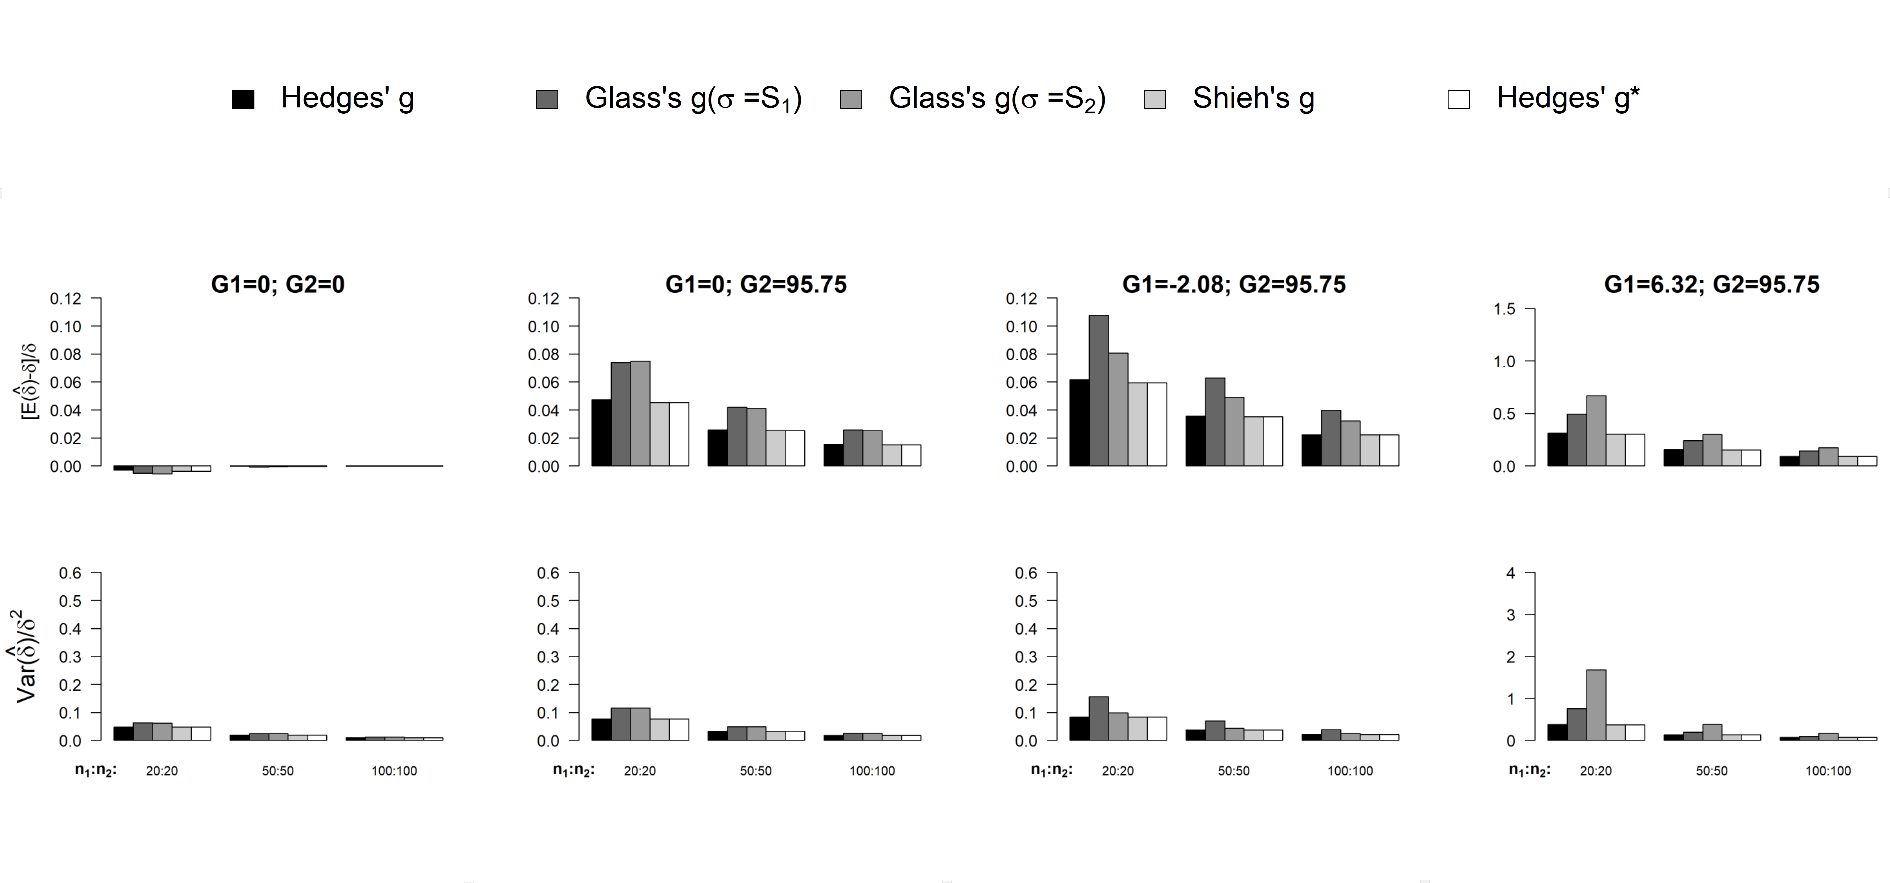
\includegraphics{D:/Documents/Github_projects/Effect-sizes/Scripts outputs/Quality of ES measures/Graphs/Unbiased estimators/Combined Figures_relative quality/Hom_bal} 

}

\caption{Bias and efficiency of estimators of standardized mean difference, when variances and sample sizes are equal across groups (condition a)}\label{fig:idHombal}
\end{sidewaysfigure}

\begin{sidewaysfigure}

{\centering 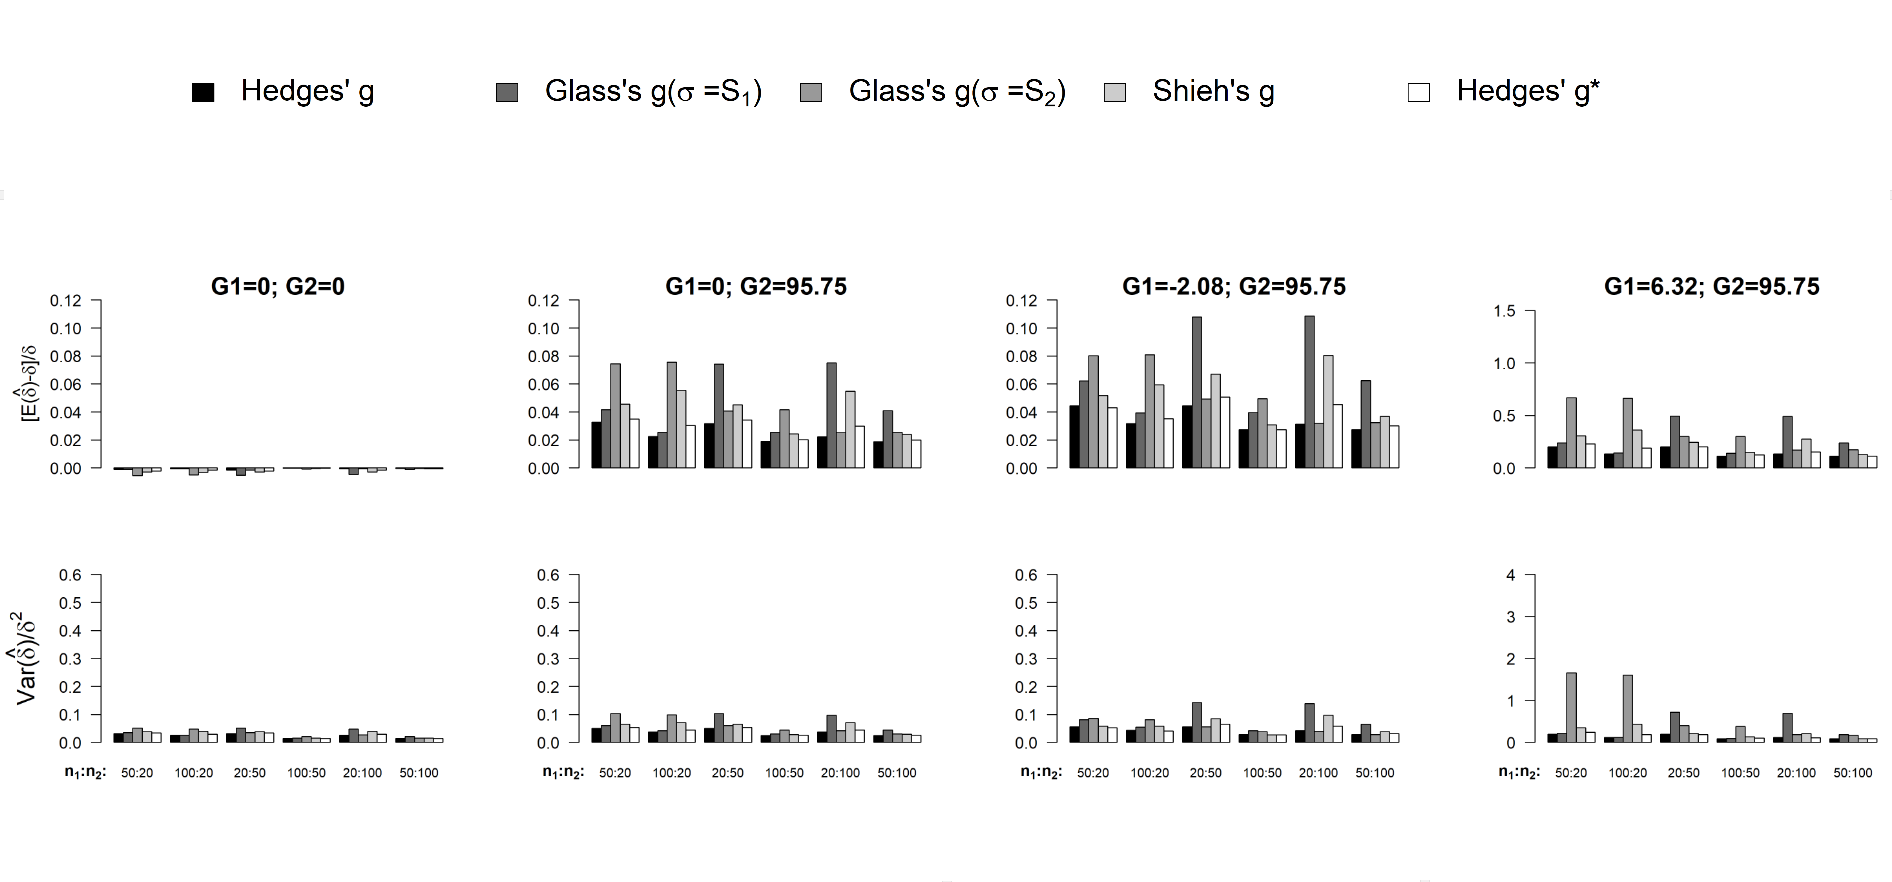
\includegraphics{D:/Documents/Github_projects/Effect-sizes/Scripts outputs/Quality of ES measures/Graphs/Unbiased estimators/Combined Figures_relative quality/Hom_unbal} 

}

\caption{Bias and efficiency of estimators of standardized mean difference, when variances are equal across groups and sample sizes are unequal (condition b)}\label{fig:idHomunbal}
\end{sidewaysfigure}

Figures \ref{fig:idHombal} and \ref{fig:idHomunbal} represent configurations where the equality of variances assumption is met. According to our expectations, one observes that the bias of all estimators is approximately zero as long as the normality assumption is met (first column in both Figures)\footnote{When looking at the relative bias for all estimators, the maximum departure from zero is 0.0064 when sample sizes are equal across groups, and 0.0065 with unequal sample sizes.}. However, the further from the normality assumption (i.e.~when moving from left to right in Figures), the larger the bias.

Figure \ref{fig:idHombal} illustrates scenarios where both population variances and sample sizes are equal across groups (condition a). One can first notice that all estimators are consistent, as their bias and variance decrease when the total sample size increase. For any departure from the normality assumption, both bias and variance of Hedges' \(g_s\), Shieh's \(d_s\) and Hedges' \(g'_s\) are similar\footnote{While the bias and variance of Cohen's $d_s$, Cohen's $d'_s$ and Shieh's $d_s$ are identical, the bias and variance of Hedges' $g_s$ is marginally different than the bias and variance of Hedges' $g'_s$ and Shieh's $g_s$ (these last two having identical bias and variance). Indeed, because of the sampling error, differences remain between sample variances, even when population variances are equal groups. Because the Hedges' correction applied to Cohen's $d_s$ does not imply the sample variances (unlike the one applied on both other estimators), the bias and variance of Hedges' $g_s$ is slighly different than the bias and variance of Hedges' $g'_s$ and Shieh's $g_s$} and smaller than the bias and variance of glass's \(g_s\) estimates using either \(S_1\) or \(S_2\) as standardizer. Moreover, when samples are extracted from skewed distributions, Glass's \(g_s\) will show different bias and variance as a function of the chosen standardizer (\(S_1\) or \(S_2\)), even if both \(S_1\) and \(S_2\) are estimates of the same population variance, based on the same sample size. This is due to non-null correlations of opposite sign between the mean difference (\(\bar{X_1}-\bar{X_2}\)) and respectively \(S_1\) and \(S_2\). For interested reader, when a non nul correlation occurs between the sample means difference (\(\bar{X_1}-\bar{X_2}\)) and the standardizer of compared estimators as well as the way this correlation impacts the bias and variance of estimators is detailed in Supplemental Material 3.

Figure \ref{fig:idHomunbal} illustrates scenarios where population variances are equal across groups and sample sizes are unequal (condition b). For any departures from the normality assumptions, Hedges' \(g_s\) shows the smallest bias and variance. Hedges' \(g_s\) and Hedges' \(g'_s\) are consistent estimators (i.e.~the larger the sample sizes, the lower the bias and the variance), unlike Shieh's \(g_s\) and Glass's \(g_s\). The bias of Glass's \(g_s\) does not depend either on the size of the experimental group or on the total sample size. The only way to decrease the bias of Glass's \(g_s\) is therefore to add subjects in the control group. On the other hand, the variance of Glass's \(g_s\) depends on both sample sizes, but not in an equivalent way: in order to reduce the variance, it is much more efficient to add subjects in the control group and when the size of the experimental group decreases so does the variance, even when the total sample size is increased. Regarding Shieh's \(g_s\), for a given sample size ratio,the bias and variance will decrease when sample sizes increase. However, there is a large effect of the sample sizes ratio in order that when the sample sizes ratio moves away from 1 by adding subjects, bias and variance might increase.\footnote{Regarding variance, in Supplemental Material 1, we mentioned that when the population effect size is nul, the larger the total sample size, the lower the variance, whatever the sample sizes ratio is constant or not. We also mentioned that this is no longer true when the population effect size is not zero and in our simulations, the effect size is never zero. The effect size effect is partially visible in Figure \ref{fig:idHomunbal} because we do not entirely remove the effect size effect when we divide the variance by $\delta^2$. This is due to the fact that one term, in the equation of the variance computation, does not depend on the effect size.} On the other side, when the sample sizes ratio moves closer to 1 by adding subjects, the bias will decrease.

When samples are extracted from skewed distributions and have unequal sizes (i.e.~\(n_1 \neq n_2\), the two last columns in Figure \ref{fig:idHomunbal}), for a constant total sample size, \(Glass's \; g_s\), Shieh's \(g_s\) and Hedges' \(g_s\) will show different bias and variance depending on which group is the largest one (e.g.~when distributions are right-skewed, the bias and variance of all these estimators when \(n_1\) and \(n_2\) are respectively 50 and 20 are not the same as their bias and variance when \(n_1\) and \(n_2\) are respectively 20 and 50). This is due to a non-null correlations of opposite sign between the mean difference (\(\bar{X_1}-\bar{X_2}\)) and their respective standardizers depending on which group is the largest one, as detailed in Supplemental Material 3. One observes that under these configurations, the bias and variance of Glass's \(g_s\) are sometimes a bit smaller and sometimes much larger than the bias and variance of Shieh's \(g_s\) and Cohen's \(d'_s\). \footnote{We learn from Supplemental Material 3 that when the $\mu_1-\mu_2 >0$ (like in our simulations), all other parameters being equal, an estimator is always less biased and variable when choosing a standardizer that is positively correlated with $\bar{X_1}-\bar{X_2}$. We also learn from Supplemental Material 3 that the smaller $n_c$, the larger the magnitude of correlation between $s_c$ and $\bar{X_1}-\bar{X_2}$. When $cor(S_c,\bar{X_1}-\bar{X_2})$ is positive, the positive effect of increasing the magnitude of the correlation is counterbalanced by the negative effect of reducing $n_c$. On the other hand, when $cor(S_c,\bar{X_1}-\bar{X_2})$ is negative, the negative effect of increasing the magnitude of the correlation is amplified by the negative effect of decreasing $n_c$. This explain why the difference between Glass's $g_s$ and other estimators is larger when Glass's $g_s$ is the least efficient estimator.}

In conclusion, Glass's \(g_s\) should always be avoided when the equality of variance assumption is met. Hedge's \(g_s\), Hedges' \(g'_s\) and Shieh's \(g_s\) are equally performant as long as the sample size ratio is close to 1. However, when designs are highly unbalanced, Shieh's \(g_s\) is not consistent anymore. While Hedge's \(g'_s\) is consistent, Hedges's \(g_s\) remains a better estimator.

\hypertarget{when-variances-are-unequal-across-groups}{%
\subparagraph{When variances are unequal across groups}\label{when-variances-are-unequal-across-groups}}

\begin{sidewaysfigure}

{\centering 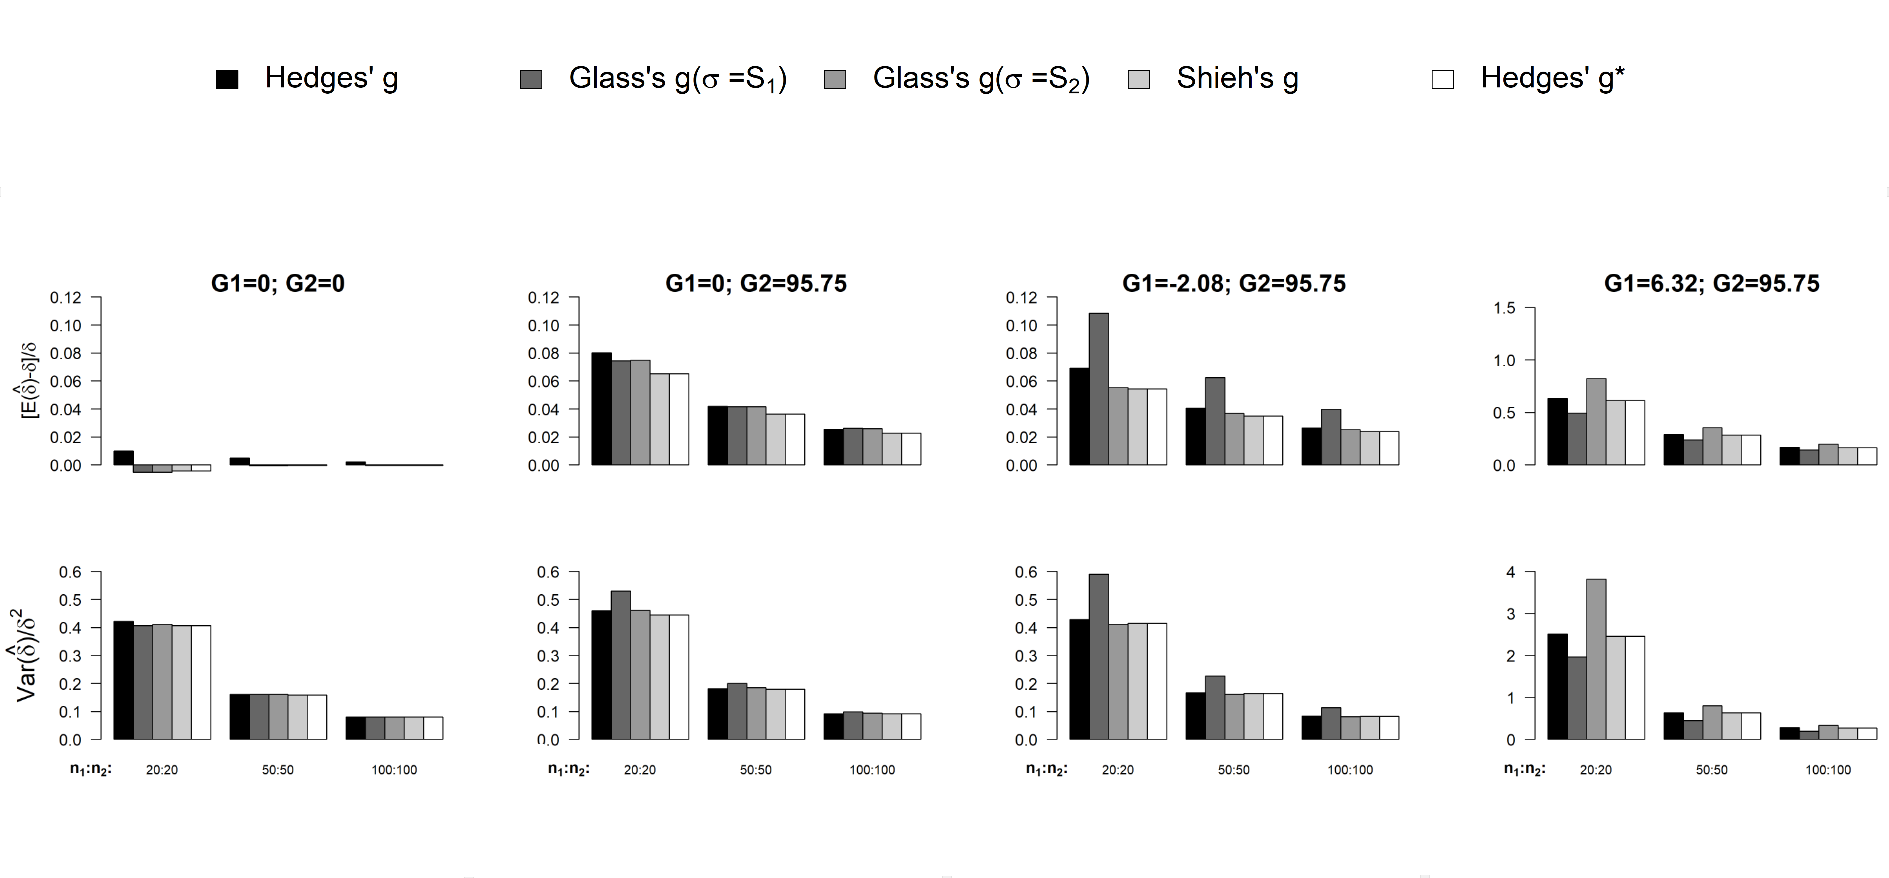
\includegraphics{D:/Documents/Github_projects/Effect-sizes/Scripts outputs/Quality of ES measures/Graphs/Unbiased estimators/Combined Figures_relative quality/Het_bal_N} 

}

\caption{Bias and efficiency of estimators of standardized mean difference, when variances are unequal across groups and sample sizes are equal (condition c), as a function of $n$-ratio}\label{fig:idHetbal1}
\end{sidewaysfigure}

\begin{sidewaysfigure}

{\centering 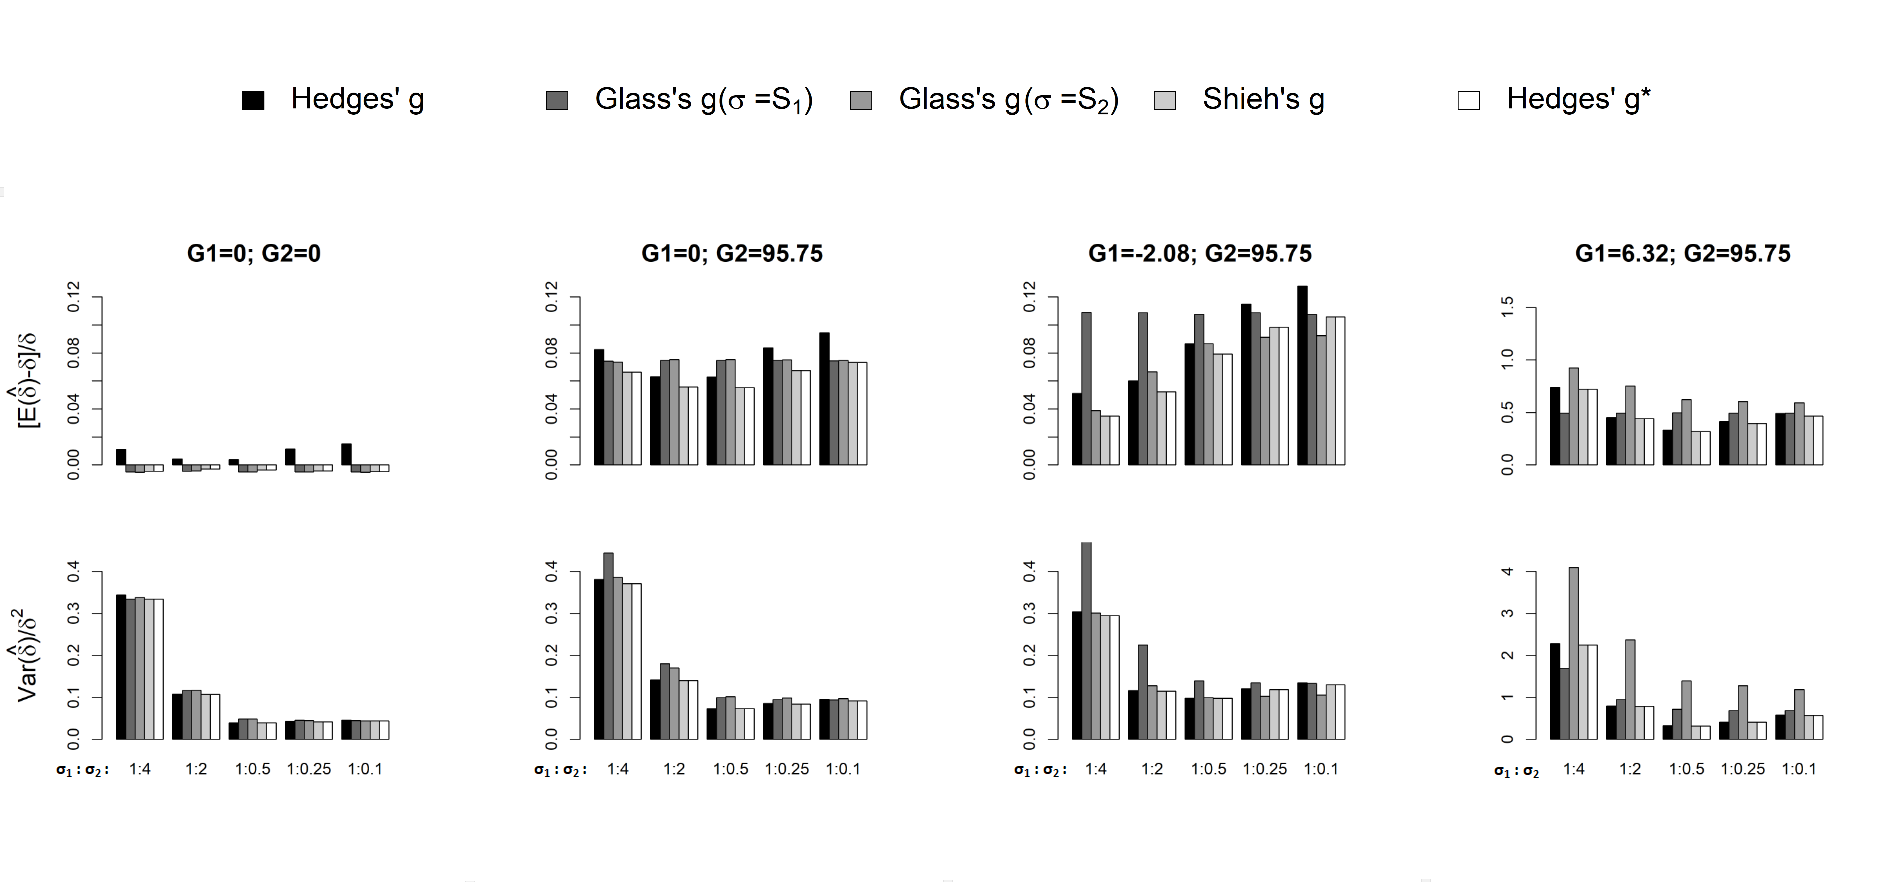
\includegraphics{D:/Documents/Github_projects/Effect-sizes/Scripts outputs/Quality of ES measures/Graphs/Unbiased estimators/Combined Figures_relative quality/Het_bal_sd} 

}

\caption{Bias and efficiency of estimators of standardized mean difference, when variances are unequal across groups and sample sizes are equal (condition c) as a function of the $SD$-ratio (when $n_1=n_2=100$)}\label{fig:idHetbal2}
\end{sidewaysfigure}

\begin{sidewaysfigure}

{\centering 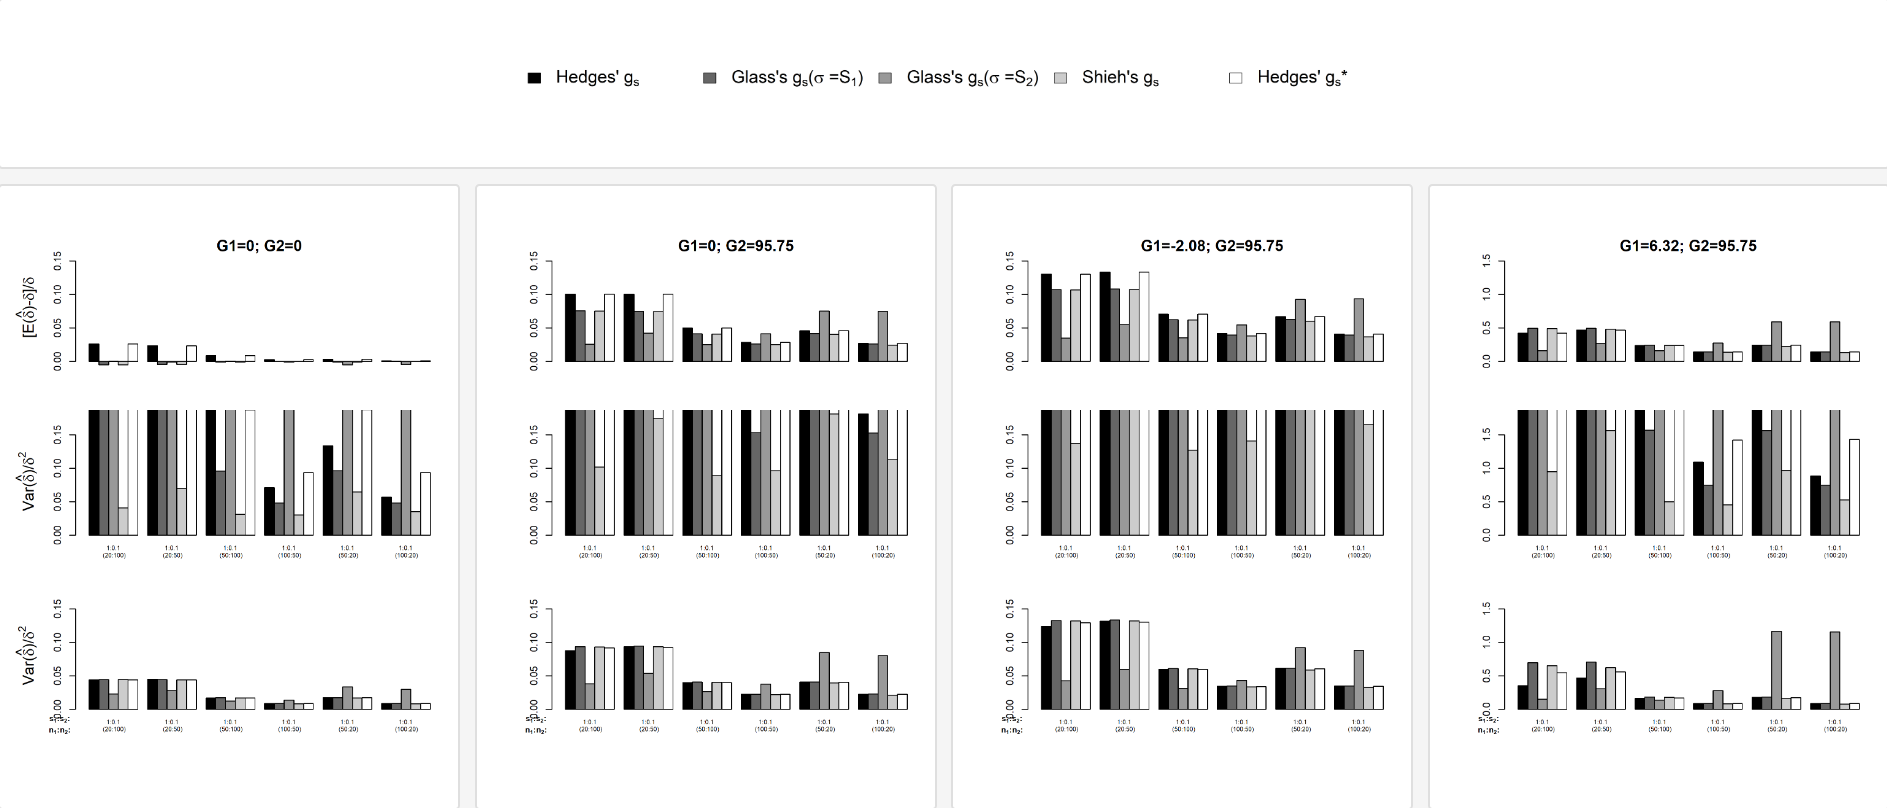
\includegraphics{D:/Documents/Github_projects/Effect-sizes/Scripts outputs/Quality of ES measures/Graphs/Unbiased estimators/Combined Figures_relative quality/Het_firstlarger_SDR10} 

}

\caption{Bias and efficiency of estimators of standardized mean difference, when variances and sample sizes are unequal across groups (condition d), total sample (N) equals 150, and $n_1>n_2$}\label{fig:idHetunbal1}
\end{sidewaysfigure}

\begin{sidewaysfigure}

{\centering 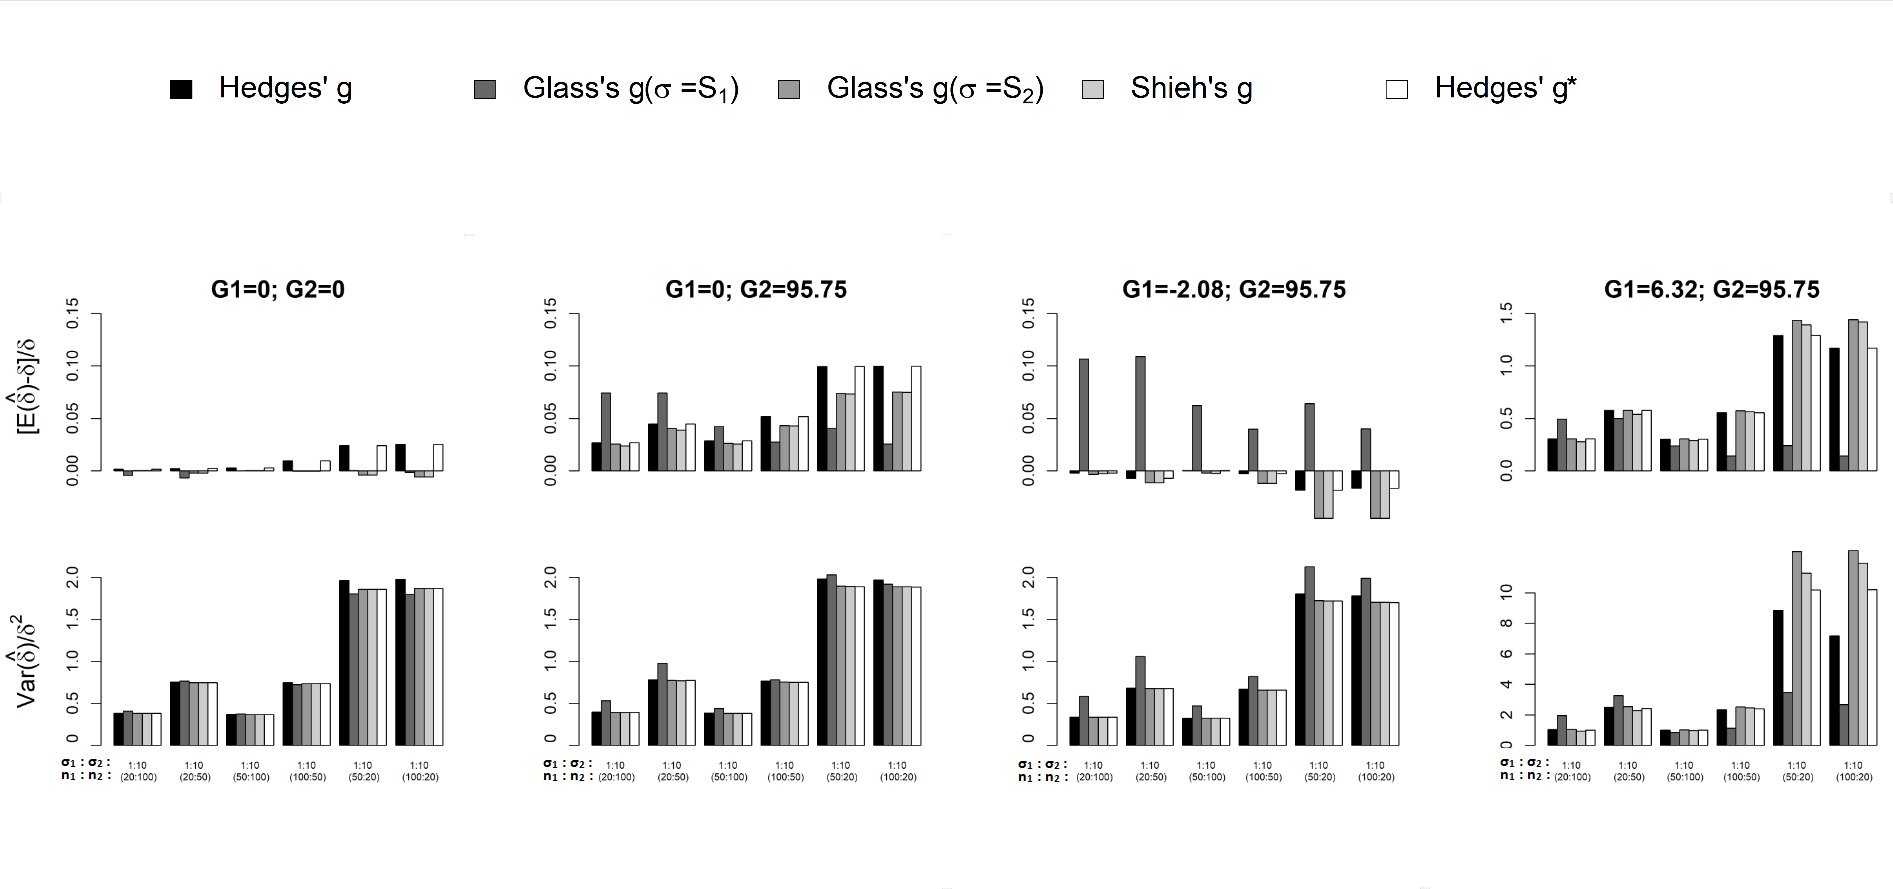
\includegraphics{D:/Documents/Github_projects/Effect-sizes/Scripts outputs/Quality of ES measures/Graphs/Unbiased estimators/Combined Figures_relative quality/Het_firstsmaller_SDR10} 

}

\caption{Bias and efficiency of estimators of standardized mean difference, when variances and sample sizes are unequal across groups (condition d), total sample (N) equals 150, and $n_1<n_2$}\label{fig:idHetunbal2}
\end{sidewaysfigure}

\begin{sidewaysfigure}

{\centering 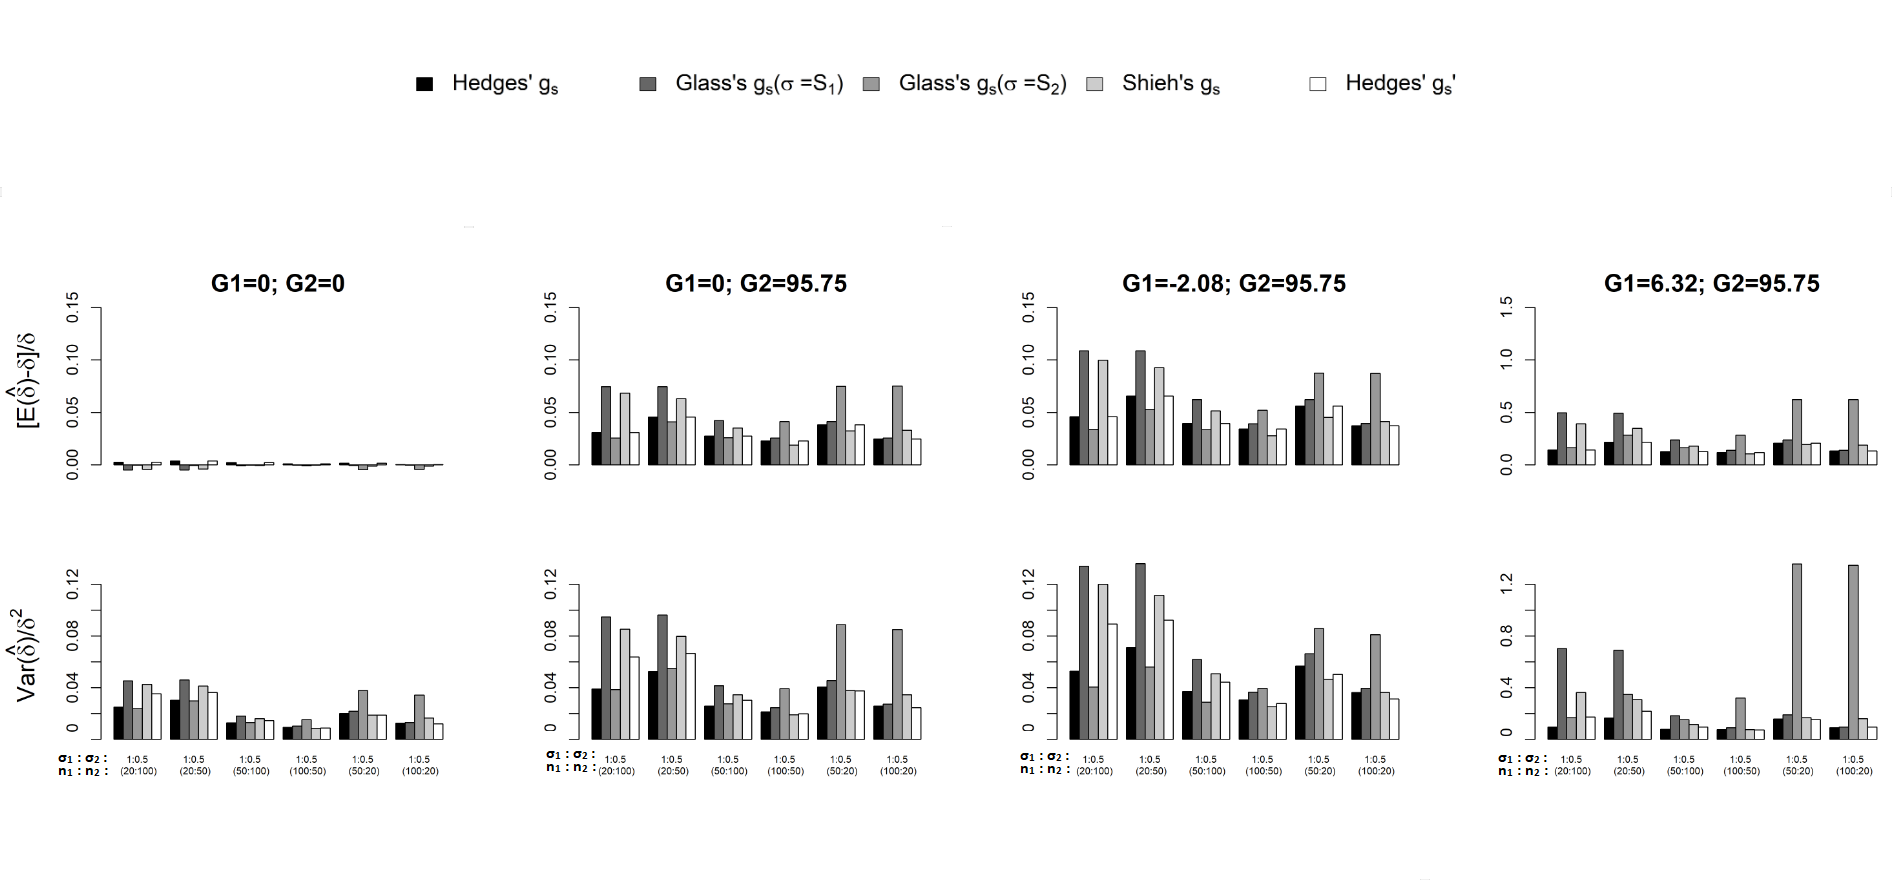
\includegraphics{D:/Documents/Github_projects/Effect-sizes/Scripts outputs/Quality of ES measures/Graphs/Unbiased estimators/Combined Figures_relative quality/Het_firstlarger_SDR2} 

}

\caption{Bias and efficiency of estimators of standardized mean difference, when variances and sample sizes are unequal across groups (condition d), total sample (N) equals 120, and $n_1>n_2$}\label{fig:idHetunbal3}
\end{sidewaysfigure}

\begin{sidewaysfigure}

{\centering 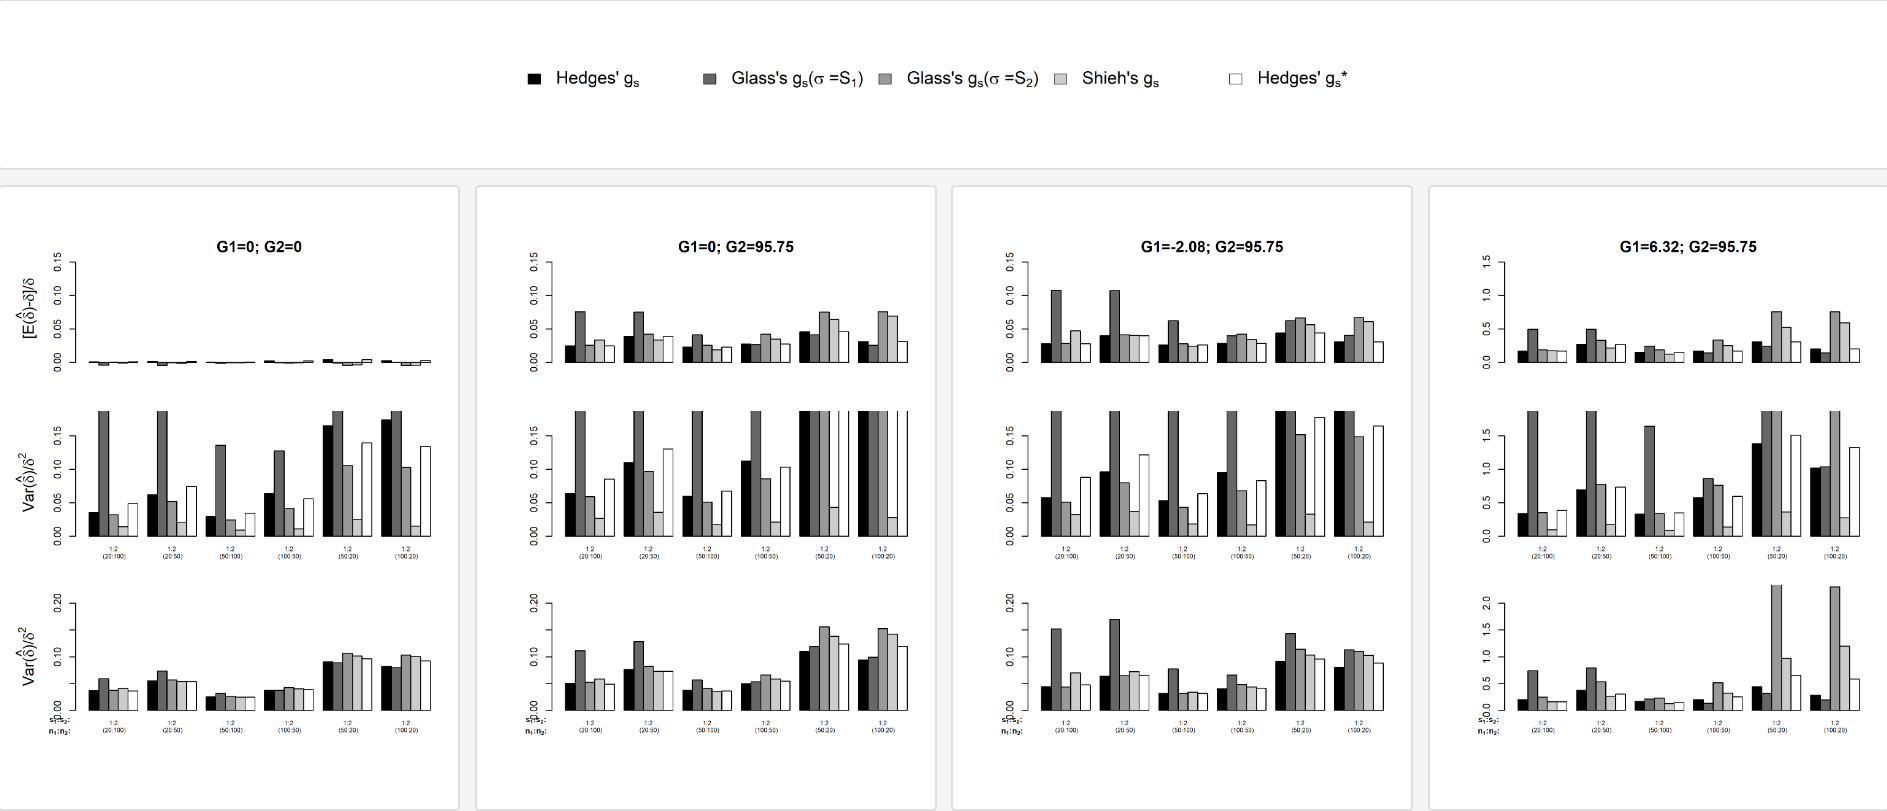
\includegraphics{D:/Documents/Github_projects/Effect-sizes/Scripts outputs/Quality of ES measures/Graphs/Unbiased estimators/Combined Figures_relative quality/Het_firstsmaller_SDR2} 

}

\caption{Bias and efficiency of estimators of standardized mean difference, when variances and sample sizes are unequal across groups (condition d), total sample (N) equals 120, and $n_1<n_2$}\label{fig:idHetunbal4}
\end{sidewaysfigure}

Figures \ref{fig:idHetbal1} to \ref{fig:idHetunbal4} represent configurations where the equality of variances assumption is not met. According to our expectations, one observes that the bias of all estimators is approximately zero as long as the normality assumption is met (first column in the three Figures), and the further from the normality assumption (i.e.~when moving from left to right in Figures), the larger the bias\footnote{When looking at the relative bias for all estimators, the maximum departure from zero is 0.0173 when sample sizes are equal across groups, and 0.0274 when both sample sizes and variances differ across groups.}. You might find it surprising that the bias of Hedges' \(g_s\) remain very small troughout these conditions. As reminded in the section \enquote{Different measures of effect size}, Hedges' \(g_s\) should be avoided when population variances and sample sizes are unequal across groups, because of the pooled error term. When pooling the estimates of two unequal population variances, the resulting estimator will be lower (in case of positive pairing) or larger (in case of negative pairing) as it should be. At the same time, when pooling two unequal population variances, the population effect size will also be lower (in case of positive pairing) or larger (in case of negative pairing) as it should be. As a consequence, the distorsion cannot be seen through the difference between the expected estimator and the population effect size measure. For this reason, the bias and variance of Hedges' \(g_s\) will not be taken into account in the following comparisons.

Figures \ref{fig:idHetbal1} and \ref{fig:idHetbal2} are dedicated to scenarios where population variances are unequal between groups and sample sizes are equal (condition c). In Figure \ref{fig:idHetbal1}, scenarios are subdivided as a function of the sample sizes and one can notice that all estimators are consistent, as their bias and variance decrease when the total sample size increases. In Figure \ref{fig:idHetbal2}, scenarios are subdivided as a function of the \(SD\)-ratio. Because the comparison pattern remains very similar for all sample sizes, we present only scenarios when sample sizes equal 20. One should first notice that for all estimators in Figure \ref{fig:idHetbal2}, the relative variance seems to be much larger when \(S_2>S_1\). This information should not be taken into account because it is only an artefact of our simulation conditions combined with the way we computed the relative variance. \footnote{We previously mentioned that when dividing the variance by $\delta^2$, we do not entirely remove the effect size effect. Actually, we introduce $\delta^2$ in the denominator of the first term, in the equation of the variance computation. Because we performed our simulations in order that $\sigma_1$ always equals 1, the smaller $S_2$, the larger the population effect size and therefore, the lower the relative variance.}
One observes that the bias and variance of both Shieh's \(g_s\) and Hedges' \(g'_s\) are identical, for any departures from the normality assumption, because sample sizes are equal across groups. The bias of Shieh's \(g_s\) (and then the bias of Hedges' \(g'_s\)) depends on the \(SD\)-ratio in order that the larger the difference between \(\sigma_1\) and \(\sigma_2\), the larger the bias. On the other side, the bias of Glass's \(g_s\) does not depend on the \(SD\)-ratio. It is always a bit larger than the bias of Shieh's \(g_s\) (and Hedges' \(g'_s\)), but the difference decreases when \(SD\)-ratio get larger \(\left(i.e. \; \;\frac{\sigma_1}{\sigma_2} = 10 \; or \; 0.1\right)\). While the bias of Glass's \(g_s\) does not depend on the \(SD\)-ratio, its variance decreases when the \(SD\)-ratio increases (i.e.~when \(S_C\) get larger, in comparison with \(S_e\)). This explains why the larger the \(SD\)-ratio, the larger the difference between the variance Glass's \(g_s\) using either \(S_1\) or \(S_2\) as standardizer. Regarding, Shieh's \(g_s\) and Hedges' \(g_s\), their variance get larger when the \(SD\)-ratio goes further from 1.

When samples are extracted from skewed distributions, the bias and variance of Glass's \(g_s\) are sometimes smaller and sometimes larger than the bias of Shieh's \(g_s\) and Hedges' \(g_s\). This is mainly due to the fact that when two samples of same sizes are extracted from two skewed distributions with unequal variances (i.e.~\(\sigma_1 \neq\sigma_2\), the two last columns in Figure \ref{fig:idHetbal2}), there will be non-null correlations of opposite sign between the mean difference (\(\bar{X_1}-\bar{X_2}\)) and the standardizer of \emph{all} estimators, depending on which population variance is the largest one \footnote{When population variances are unequal, a non-null correlation occurs between standardizers estimates and $\bar{X_1}-\bar{X_2}$. For standardizers computed based on both $S_1$ and $S_2$, the sign of the correlation between the standardizer and the means difference will be the same as the sign of the correlation between the mean difference and the estimate of the larger population variance. For interested readers, this is detailed in Supplemental Material 3.}.

Figures \ref{fig:idHetunbal1} to \ref{fig:idHetunbal4} are dedicated to scenarios where both samples sizes and population variances differ across groups. Due to a high number of combinations between the sample sizes-ratio and the variances-ratio in our simulations, we decided to present only some conditions. Because equations in Table 3 revealed an interaction effect between the sample sizes ratio and the \(SD\)-ratio on the bias and variance of Hedges' \(g_s\) and Shieh's \(g_s\) (see Supplemental Material 1), we chose to present all configurations where the larger \(SD\) is 10 times larger than the smaller \(SD\) (Figures \ref{fig:idHetunbal1} and \ref{fig:idHetunbal2}), and configurations where the larger \(SD\) is twice larger than the smaller \(SD\) (Figures \ref{fig:idHetunbal3} and \ref{fig:idHetunbal4}), in order to compare the effect of the sample sizes ratio on the bias and variance of all estimators when the \(SD\)-ratio is large (\(\frac{\sigma_1}{\sigma_2}=10 \; or \; .1\) ) or medium (\(\frac{\sigma_1}{\sigma_2}=2 \; or \; .5\)).

When distributions are symmetric, the bias of Glass's \(g_s\) only depends on the size of the control group and is therefore not impacted by neither the sample sizes ratio nor the total sample size. When comparing Figures \ref{fig:idHetunbal1} to \ref{fig:idHetunbal4}, one can also notice that the bias of Glass's \(g_s\) does not depend on the \(SD\)-ratio either. Unlike the bias of Glass's \(g'_s\), its variance depends on both sample sizes, but not in an equivalent way: most of the time, it is more efficient, in order to reduce the variance of Glass's \(g_s\), to add subjects in the control group. Regarding Hedges' \(g_s\) and Shieh's \(g'_s\), their respective biases and variances depend on an interaction effect between the sample sizes ratio and the \(SD\)-ratio \(\left( \frac{n_1}{n_2} \times \frac{\sigma_1}{\sigma_2} \right)\): the sample sizes ratio associated with the smallest bias and variance is not the same when the more variable group is 10 times more variable than the other group (Figures \ref{fig:idHetunbal1} and \ref{fig:idHetunbal2}) than when it is only twice more variable (Figures \ref{fig:idHetunbal3} and \ref{fig:idHetunbal4}). However, it is always true that the respective biases and variances of Hedges' \(g_s\) and Shieh's \(g_s\) are always smaller when there is a positive pairing between sample sizes and variances. When samples are extracted from skewed distributions, the bias and variance of Glass's \(g_s\) are sometimes smaller and sometimes larger than the bias of Shieh's \(g_s\) and Hedges' \(g_s\), due to a combination of three factors: (1) which group is the largest one, (2) which group has the smallest standard deviation and (3) what is the correlation between the standardizer and the means difference.

In summary, when variances are unequal across populations, Glass's \(g_s\) is sometimes better but also sometimes much worst than respectively Shieh's \(g_s\) and Hedges' \(g'_s\). The performance of Glass's \(g_s\) highly depends on parameters that we cannot control (i.e.~an triple interaction) and for this reason, we do not recommend using it. When designs are not \enquote{too unbalanced}, Shieh's \(g_s\) and Hedges' \$g'\_s" are both appropriate but the further the sample sizes ratio is from 1, the larger the bias of Shieh's \(g_s\) in order that in the end, our favourite measure is Hedges' \$g'\_s".

\hypertarget{conclusion}{%
\paragraph{Conclusion}\label{conclusion}}

TO DO

\hypertarget{refs}{}
\leavevmode\hypertarget{ref-Algina_et_al_2006}{}%
Algina, J., Keselman, H. J., \& Penfield, R. D. (2006). Confidence intervals for an effect size when variances are not equal. \emph{Journal of Modern Applied Statistical Methods}, \emph{5}(1), 1--13. doi:\href{https://doi.org/10.22237/jmasm/1146456060}{10.22237/jmasm/1146456060}

\leavevmode\hypertarget{ref-Altman_2005}{}%
Altman, G. D. (2005). Why we need confidence intervals. \emph{World Journal of Surgery}, \emph{29}, 554--556. doi:\href{https://doi.org/10.1007/s00268-005-7911-0}{10.1007/s00268-005-7911-0}

\leavevmode\hypertarget{ref-AERA_2006}{}%
American Educational Research Association. (2006). Standards for reporting on empirical social science research in aera publications. \emph{Educational Researcher}, \emph{35}, 33--40. doi:\href{https://doi.org/10.3102/0013189X035006033}{10.3102/0013189X035006033}

\leavevmode\hypertarget{ref-APA_2010}{}%
American Psychological Association. (2010). \emph{Publication manual of the american psychological association {[}apa{]} (6 ed.)} (American Psychological Association.). Washington, DC:

\leavevmode\hypertarget{ref-Andersen_et_al_2007}{}%
Andersen, M. B., McCullagh, P., \& Wilson, G. J. (2007). But what do the numbers really tell us? Arbitrary metrics and effect size reporting in sport psychology research. \emph{Journal of Sport \& Exercise Psychology}, \emph{29}, 664--672.

\leavevmode\hypertarget{ref-Bothe_Richardson_2011}{}%
Bothe, A. K., \& Richardson, J. D. (2011). Statistical, practical, clinical, and personal significance: Definitions and applications in speech-language pathology. \emph{American Journal of Speech-Language Pathology}, \emph{20}, 233--242.

\leavevmode\hypertarget{ref-Cain_et_al_2017}{}%
Cain, M. K., Zhang, Z., \& Yuan, K.-H. (2017). Univariate and multivariate skewness and kurtosis for measuring nonnormality: Prevalence, influence and estimation. \emph{Behavior Research Methods}, \emph{49}(5), 1716--1735. doi:\href{https://doi.org/10.3758/s13428-016-0814-1}{10.3758/s13428-016-0814-1}

\leavevmode\hypertarget{ref-Coe_2002}{}%
Coe, R. (2002). \emph{It's the effect size, stupid. What effect size is and why it is important}. Retrieved from \url{https://www.leeds.ac.uk/educol/documents/00002182.htm}

\leavevmode\hypertarget{ref-Cohen_1965}{}%
Cohen, J. (1965). Some statistical issues in psychological research. In \emph{Handbook of clinical psychology} (B. B. Wolman., pp. 95--121). New York: McGraw-Hill.

\leavevmode\hypertarget{ref-Cumming_2013}{}%
Cumming, G. (2013). Cohen's d needs to be readily interpretable: Comment on shieh (2013). \emph{Behavior Research Methods}, \emph{45}, 968--971. doi:\href{https://doi.org/10.3758/s13428-013-0392-4}{10.3758/s13428-013-0392-4}

\leavevmode\hypertarget{ref-Delacre_et_al_2017}{}%
Delacre, M., Lakens, D., \& Leys, C. (2017). Why psychologists should by default use welch's t-test instead of student's t-test. \emph{International Review of Social Psychology}, \emph{30}(1), 92--101. doi:\href{https://doi.org/10.5334/irsp.82}{10.5334/irsp.82}

\leavevmode\hypertarget{ref-Delacre_et_al_2019}{}%
Delacre, M., Leys, C., Mora, Y. L., \& Lakens, D. (2019). Taking parametric assumptions seriously: Arguments for the use of welch's f-test instead of the classical f-test in one-way anova. \emph{International Review of Social Psychology}, \emph{32}(1), 1--12. doi:\href{https://doi.org/http://doi.org/10.5334/irsp.198}{http://doi.org/10.5334/irsp.198}

\leavevmode\hypertarget{ref-Ellis_2015}{}%
Ellis, P. D. (2015). \emph{The Essential Guide to Effect Sizes: Statistical Power, Meta-Analysis, and the Interpretation of Research Results} (Cambridge University Press.). Cambridge, UK.

\leavevmode\hypertarget{ref-Erceg-Hurn_Mirosevich_2008}{}%
Erceg-Hurn, D. M., \& Mirosevich, V. M. (2008). Modern robust statistical methods: An easy way to maximize the accuracy and power of your research. \emph{American Psychologist}, \emph{63}(7), 591--601. doi:\href{https://doi.org/10.1037/0003-066X.63.7.591}{10.1037/0003-066X.63.7.591}

\leavevmode\hypertarget{ref-Fan_2001}{}%
Fan, X. (2001). Statistical significance and effect size in education research: Two sides of a coin. \emph{Journal of Educational Research}, \emph{94}(5), 275--282. doi:\href{https://doi.org/10.1080/00220670109598763}{10.1080/00220670109598763}

\leavevmode\hypertarget{ref-Glass_et_al_1981}{}%
Glass, G. V., McGav, B., \& Smith, M. L. (2005). \emph{Meta-analysis in social research} (Sage.). Beverly Hills, CA.

\leavevmode\hypertarget{ref-Glass_et_al_1972}{}%
Glass, G. V., Peckham, P. D., \& Sanders, J. R. (1972). Consequences of failure to meet assumptions underlying the fixed effects analyses of variance and covariance. \emph{Review of Educational Research}, \emph{42}(3), 237--288. doi:\href{https://doi.org/10.3102/00346543042003237}{10.3102/00346543042003237}

\leavevmode\hypertarget{ref-Grissom_2000}{}%
Grissom, R. J. (2000). Heterogeneity of variance in clinical data. \emph{Journal of Consulting and Clinical Psychology}, \emph{68}(1), 155--165. doi:\href{https://doi.org/10.1037//0022-006x.68.1.155}{10.1037//0022-006x.68.1.155}

\leavevmode\hypertarget{ref-Grissom_Kim_2001}{}%
Grissom, R. J., \& Kim, J. J. (2001). Review of assumptions and problems in the appropriate conceptualization of effect size. \emph{Psychological Methods}, \emph{6}(2), 135--146. doi:\href{https://doi.org/10.1037/1082-989X.6.2.135}{10.1037/1082-989X.6.2.135}

\leavevmode\hypertarget{ref-Grissom_and_Kim_2012}{}%
Grissom, R. J., \& Kim, J. J. (2012). \emph{Effect size for research} (Routledges.). New York, NY.

\leavevmode\hypertarget{ref-Grissom_and_kim_2005}{}%
Grissom, R. R., \& Kim, J. J. (2005). \emph{Effect size for research: A broad practical approach.} (Lawrence Erlbaum Associates, Mahwah, N.J.). London.

\leavevmode\hypertarget{ref-Hays_1963}{}%
Hays, W. L. (1963). \emph{Statistics for psychologists} (Holt, Rinehart \& Winston.). New York.

\leavevmode\hypertarget{ref-Hedges_Olkin_1985}{}%
Hedges, L. V., \& Olkin, I. (1985). \emph{Statistical methods for meta-analysis} (Academic Press.). Cambridge, Massachusetts. doi:\href{https://doi.org/10.1016/C2009-0-03396-0}{10.1016/C2009-0-03396-0}

\leavevmode\hypertarget{ref-Henson_Smith_2000}{}%
Henson, R. I., \& Smith, A. D. (2000). State of the art in statistical significance and effect size reporting: A review of the APA task force report and current trends. \emph{Journal of Research and Development in Education}, \emph{33}(4), 285--296.

\leavevmode\hypertarget{ref-Huynh_1989}{}%
Huynh, C.-L. (1989). A unified approach to the estimation of effect size in meta-analysis. San Francisco: Paper presented at the Annual Meeting of the American Educational Research Association.

\leavevmode\hypertarget{ref-Kelley_2005}{}%
Kelley, K. (2005). The effects of nonnormal distributions on confidence intervales around the standardized mean difference: Bootstrap and parametric confidence intervals. \emph{Educational and Psychological Measurement}, \emph{65}(1), 51--69. doi:\href{https://doi.org/10.1177/0013164404264850}{10.1177/0013164404264850}

\leavevmode\hypertarget{ref-Keselman_et_al_2008}{}%
Keselman, H. J., Algina, J., Lix, L. M., Deering, K. N., \& Wilcox, R. R. (2008). A generally robust approach for testing hypotheses and setting confidence intervals for effect sizes. \emph{Psychological Methods}, \emph{13}(2), 110--129. doi:\href{https://doi.org/10.1037/1082-989X.13.2.110}{10.1037/1082-989X.13.2.110}

\leavevmode\hypertarget{ref-Kirk_2009}{}%
Kirk, R. E. (2009). Practical significance: A concept whose time has come. \emph{Educational and Psychological Measurement}, \emph{56}(5), 746--759. doi:\href{https://doi.org/10.1177/0013164496056005002\%20}{10.1177/0013164496056005002 }

\leavevmode\hypertarget{ref-Kulinskaya_Staudte_2007}{}%
Kulinskaya, E., \& Staudte, R. G. (2007). Confidence intervals for the standardized effect arising in the comparison of two normal populations. \emph{Statistics In Medicine}, \emph{26}, 2853--2871. doi:\href{https://doi.org/10.1002/sim.2751}{10.1002/sim.2751}

\leavevmode\hypertarget{ref-Lakens_2013}{}%
Lakens, D. (2013). Calculating and reporting effect sizes to facilitate cumulative science: A practical primer for t-tests and ANOVAs. \emph{Frontiers in Psychology}, \emph{4}(863), 1--12. doi:\href{https://doi.org/10.3389/fpsyg.2013.00863}{10.3389/fpsyg.2013.00863}

\leavevmode\hypertarget{ref-Li_2016}{}%
Li, J. (2016). Effect size measures in a two-independent-samples case with nonnormal and nonhomogeneous data. \emph{Behavior Research Methods}, \emph{48}(4), 1560--1574. doi:\href{https://doi.org/10.3758/s13428-015-0667-z}{10.3758/s13428-015-0667-z}

\leavevmode\hypertarget{ref-McBride_et_al_1993}{}%
McBride, G. B., Loftis, J. C., \& Adkins, N. C. (1993). What do significance tests really tell us about the environment? \emph{Environmental Management}, \emph{17}(4), 423--432.

\leavevmode\hypertarget{ref-Meehl_1990}{}%
Meehl, P. E. (1990). Appraising and amending theories: The strategy of Lakatosian defense and two principles that warrant it. \emph{Psychological Inquiry}, \emph{1}(2), 108--141.

\leavevmode\hypertarget{ref-Micceri_1989}{}%
Micceri, T. (1989). The unicorn, the normal curve, and other improbable creatures. \emph{Psychological Bulletin}, \emph{105}(1), 156--166. doi:\href{https://doi.org/10.1037/0033-2909.105.1.156}{10.1037/0033-2909.105.1.156}

\leavevmode\hypertarget{ref-Nakagawa_and_Cuthill_2007}{}%
Nakagawa, S., \& Cuthill, I. C. (2007). Effect size, confidence interval and statistical significance: A practical guide for biologists. \emph{Biological Reviews}, \emph{82}, 591--605. doi:\href{https://doi.org/10.1111/j.1469-185X.2007.00027.x}{10.1111/j.1469-185X.2007.00027.x}

\leavevmode\hypertarget{ref-Olejnik_Algina_2000}{}%
Olejnik, S., \& Algina, J. (2000). Measures of effect size for comparative studies: Applications, interpretations, and limitations. \emph{Contemporary Educational Psychology}, \emph{25}, 241--286. doi:\href{https://doi.org/10.1006/ceps.2000.1040}{10.1006/ceps.2000.1040}

\leavevmode\hypertarget{ref-Peng_and_Chen_2014}{}%
Peng, C.-Y., \& Chen, L.-T. (2014). Beyond cohen's d: Alternative effect size measures for between-subject designs. \emph{THE JOURNAL OF EXPERIMENTAL EDUCATION}, \emph{82}(1), 22--50. doi:\href{https://doi.org/10.1080/00220973.2012.745471}{10.1080/00220973.2012.745471}

\leavevmode\hypertarget{ref-Peng_et_al_2013}{}%
Peng, C.-Y., Chen, L.-T., Chiang, H.-M., \& Chiang, Y.-C. (2013). The Impact of APA and AERA Guidelines on Effect size Reporting. \emph{Contemporary Educational Psychology}, \emph{82}(1), 22--50. doi:\href{https://doi.org/10.1080/00220973.2012.745471}{10.1080/00220973.2012.745471}

\leavevmode\hypertarget{ref-Prentice_Miller_1992}{}%
Prentice, D., \& Miller, D. T. (1990). When small effects are impressive. \emph{Psychological Bulletin}, \emph{112}(1), 160--164.

\leavevmode\hypertarget{ref-Raviv}{}%
Raviv, E. (2014). \emph{Bias vs. Consistency}. Retrieved March 25, 2020, from \url{https://eranraviv.com/bias-vs-consistency/}

\leavevmode\hypertarget{ref-Rosenthal_1994}{}%
Rosenthal, R. (1994). Parametric measures of effect size. In H. Cooper \& L. V. Hedges (Eds.), \emph{The hand-book of research synthesis} (pp. 231--244). New-York: Sage.

\leavevmode\hypertarget{ref-Shieh_2013}{}%
Shieh, G. (2013). Confidence intervals and sample size calculations for the weighted eta-squared effect sizes in one-way heteroscedastic ANOVA. \emph{Behavior Research Methods}, \emph{45}(1), 2--37. doi:\href{https://doi.org/10.3758/s13428-012-0228-7}{10.3758/s13428-012-0228-7}

\leavevmode\hypertarget{ref-Steyn_2000}{}%
Steyn, H. S. (2000). Practical significance of the difference in means. \emph{Journal of Industrial Psychology}, \emph{26}(3), 1--3.

\leavevmode\hypertarget{ref-Stout_Ruble_1995}{}%
Stout, D. D., \& Ruble, T. L. (1995). Assessing the practical signficance of empirical results in accounting education research: The use of effect size information. \emph{Journal of Accounting Education}, \emph{13}(3), 281--298.

\leavevmode\hypertarget{ref-Sullivan_Feinn_2012}{}%
Sullivan, G., \& Feinn, R. (2012). Using effect size---or why the p value is not enough. \emph{Journal of Graduate Medical Education}, 279--282. doi:\href{https://doi.org/10.4300/JGME-D-12-00156.1}{10.4300/JGME-D-12-00156.1}

\leavevmode\hypertarget{ref-Thompson_2002}{}%
Thompson, B. (2002). "Statistical","Practical", and "Clinical": How Many Kinds of Significance Do Counselors Need to Consider? \emph{Journal of Counseling \& Development}, \emph{80}, 64--71.

\leavevmode\hypertarget{ref-Tyler_1931}{}%
Tyler, R. W. (1931). What is Statistical Significance? \emph{Educational Research Bulletin}, \emph{X}(5), 115--142.

\leavevmode\hypertarget{ref-Wackerly_et_al_2008}{}%
Wackerly, D. D., Mendenhall, W., \& Scheaffer, R. L. (2008). \emph{Mathematical statistics with applications (7th edition)} (Brooks/Cole, Cengage Learning.). Belmont, USA.

\leavevmode\hypertarget{ref-Welch_1938}{}%
Welch, B. L. (1938). The significance of the difference between two means when the population variances are unequal. \emph{Biometrika}, \emph{29}, 350--362.

\leavevmode\hypertarget{ref-Wilkinson_1999}{}%
Wilkinson, L., \& the Task Force on Statistical Inference. (1999). Statistical methods in psychology journals: Guidelines and explanations. \emph{American Psychologist}, \emph{54}(8), 594--604.

\leavevmode\hypertarget{ref-Yuan_et_al_2004}{}%
Yuan, K.-H., Bentler, P. M., \& Chan, W. (2004). Structural equation modeling with heavy tailed distributions. \emph{Psychometrika}, \emph{69}(3), 421--436. doi:\href{https://doi.org/10.1007/bf02295644}{10.1007/bf02295644}

\leavevmode\hypertarget{ref-Algina_et_al_2006}{}%
Algina, J., Keselman, H. J., \& Penfield, R. D. (2006). Confidence intervals for an effect size when variances are not equal. \emph{Journal of Modern Applied Statistical Methods}, \emph{5}(1), 1--13. doi:\href{https://doi.org/10.22237/jmasm/1146456060}{10.22237/jmasm/1146456060}

\leavevmode\hypertarget{ref-Altman_2005}{}%
Altman, G. D. (2005). Why we need confidence intervals. \emph{World Journal of Surgery}, \emph{29}, 554--556. doi:\href{https://doi.org/10.1007/s00268-005-7911-0}{10.1007/s00268-005-7911-0}

\leavevmode\hypertarget{ref-AERA_2006}{}%
American Educational Research Association. (2006). Standards for reporting on empirical social science research in aera publications. \emph{Educational Researcher}, \emph{35}, 33--40. doi:\href{https://doi.org/10.3102/0013189X035006033}{10.3102/0013189X035006033}

\leavevmode\hypertarget{ref-APA_2010}{}%
American Psychological Association. (2010). \emph{Publication manual of the american psychological association {[}apa{]} (6 ed.)} (American Psychological Association.). Washington, DC:

\leavevmode\hypertarget{ref-Andersen_et_al_2007}{}%
Andersen, M. B., McCullagh, P., \& Wilson, G. J. (2007). But what do the numbers really tell us? Arbitrary metrics and effect size reporting in sport psychology research. \emph{Journal of Sport \& Exercise Psychology}, \emph{29}, 664--672.

\leavevmode\hypertarget{ref-Bothe_Richardson_2011}{}%
Bothe, A. K., \& Richardson, J. D. (2011). Statistical, practical, clinical, and personal significance: Definitions and applications in speech-language pathology. \emph{American Journal of Speech-Language Pathology}, \emph{20}, 233--242.

\leavevmode\hypertarget{ref-Cain_et_al_2017}{}%
Cain, M. K., Zhang, Z., \& Yuan, K.-H. (2017). Univariate and multivariate skewness and kurtosis for measuring nonnormality: Prevalence, influence and estimation. \emph{Behavior Research Methods}, \emph{49}(5), 1716--1735. doi:\href{https://doi.org/10.3758/s13428-016-0814-1}{10.3758/s13428-016-0814-1}

\leavevmode\hypertarget{ref-Coe_2002}{}%
Coe, R. (2002). \emph{It's the effect size, stupid. What effect size is and why it is important}. Retrieved from \url{https://www.leeds.ac.uk/educol/documents/00002182.htm}

\leavevmode\hypertarget{ref-Cohen_1965}{}%
Cohen, J. (1965). Some statistical issues in psychological research. In \emph{Handbook of clinical psychology} (B. B. Wolman., pp. 95--121). New York: McGraw-Hill.

\leavevmode\hypertarget{ref-Cumming_2013}{}%
Cumming, G. (2013). Cohen's d needs to be readily interpretable: Comment on shieh (2013). \emph{Behavior Research Methods}, \emph{45}, 968--971. doi:\href{https://doi.org/10.3758/s13428-013-0392-4}{10.3758/s13428-013-0392-4}

\leavevmode\hypertarget{ref-Delacre_et_al_2017}{}%
Delacre, M., Lakens, D., \& Leys, C. (2017). Why psychologists should by default use welch's t-test instead of student's t-test. \emph{International Review of Social Psychology}, \emph{30}(1), 92--101. doi:\href{https://doi.org/10.5334/irsp.82}{10.5334/irsp.82}

\leavevmode\hypertarget{ref-Delacre_et_al_2019}{}%
Delacre, M., Leys, C., Mora, Y. L., \& Lakens, D. (2019). Taking parametric assumptions seriously: Arguments for the use of welch's f-test instead of the classical f-test in one-way anova. \emph{International Review of Social Psychology}, \emph{32}(1), 1--12. doi:\href{https://doi.org/http://doi.org/10.5334/irsp.198}{http://doi.org/10.5334/irsp.198}

\leavevmode\hypertarget{ref-Ellis_2015}{}%
Ellis, P. D. (2015). \emph{The Essential Guide to Effect Sizes: Statistical Power, Meta-Analysis, and the Interpretation of Research Results} (Cambridge University Press.). Cambridge, UK.

\leavevmode\hypertarget{ref-Erceg-Hurn_Mirosevich_2008}{}%
Erceg-Hurn, D. M., \& Mirosevich, V. M. (2008). Modern robust statistical methods: An easy way to maximize the accuracy and power of your research. \emph{American Psychologist}, \emph{63}(7), 591--601. doi:\href{https://doi.org/10.1037/0003-066X.63.7.591}{10.1037/0003-066X.63.7.591}

\leavevmode\hypertarget{ref-Fan_2001}{}%
Fan, X. (2001). Statistical significance and effect size in education research: Two sides of a coin. \emph{Journal of Educational Research}, \emph{94}(5), 275--282. doi:\href{https://doi.org/10.1080/00220670109598763}{10.1080/00220670109598763}

\leavevmode\hypertarget{ref-Glass_et_al_1981}{}%
Glass, G. V., McGav, B., \& Smith, M. L. (2005). \emph{Meta-analysis in social research} (Sage.). Beverly Hills, CA.

\leavevmode\hypertarget{ref-Glass_et_al_1972}{}%
Glass, G. V., Peckham, P. D., \& Sanders, J. R. (1972). Consequences of failure to meet assumptions underlying the fixed effects analyses of variance and covariance. \emph{Review of Educational Research}, \emph{42}(3), 237--288. doi:\href{https://doi.org/10.3102/00346543042003237}{10.3102/00346543042003237}

\leavevmode\hypertarget{ref-Grissom_2000}{}%
Grissom, R. J. (2000). Heterogeneity of variance in clinical data. \emph{Journal of Consulting and Clinical Psychology}, \emph{68}(1), 155--165. doi:\href{https://doi.org/10.1037//0022-006x.68.1.155}{10.1037//0022-006x.68.1.155}

\leavevmode\hypertarget{ref-Grissom_Kim_2001}{}%
Grissom, R. J., \& Kim, J. J. (2001). Review of assumptions and problems in the appropriate conceptualization of effect size. \emph{Psychological Methods}, \emph{6}(2), 135--146. doi:\href{https://doi.org/10.1037/1082-989X.6.2.135}{10.1037/1082-989X.6.2.135}

\leavevmode\hypertarget{ref-Grissom_and_Kim_2012}{}%
Grissom, R. J., \& Kim, J. J. (2012). \emph{Effect size for research} (Routledges.). New York, NY.

\leavevmode\hypertarget{ref-Grissom_and_kim_2005}{}%
Grissom, R. R., \& Kim, J. J. (2005). \emph{Effect size for research: A broad practical approach.} (Lawrence Erlbaum Associates, Mahwah, N.J.). London.

\leavevmode\hypertarget{ref-Hays_1963}{}%
Hays, W. L. (1963). \emph{Statistics for psychologists} (Holt, Rinehart \& Winston.). New York.

\leavevmode\hypertarget{ref-Hedges_Olkin_1985}{}%
Hedges, L. V., \& Olkin, I. (1985). \emph{Statistical methods for meta-analysis} (Academic Press.). Cambridge, Massachusetts. doi:\href{https://doi.org/10.1016/C2009-0-03396-0}{10.1016/C2009-0-03396-0}

\leavevmode\hypertarget{ref-Henson_Smith_2000}{}%
Henson, R. I., \& Smith, A. D. (2000). State of the art in statistical significance and effect size reporting: A review of the APA task force report and current trends. \emph{Journal of Research and Development in Education}, \emph{33}(4), 285--296.

\leavevmode\hypertarget{ref-Huynh_1989}{}%
Huynh, C.-L. (1989). A unified approach to the estimation of effect size in meta-analysis. San Francisco: Paper presented at the Annual Meeting of the American Educational Research Association.

\leavevmode\hypertarget{ref-Kelley_2005}{}%
Kelley, K. (2005). The effects of nonnormal distributions on confidence intervales around the standardized mean difference: Bootstrap and parametric confidence intervals. \emph{Educational and Psychological Measurement}, \emph{65}(1), 51--69. doi:\href{https://doi.org/10.1177/0013164404264850}{10.1177/0013164404264850}

\leavevmode\hypertarget{ref-Keselman_et_al_2008}{}%
Keselman, H. J., Algina, J., Lix, L. M., Deering, K. N., \& Wilcox, R. R. (2008). A generally robust approach for testing hypotheses and setting confidence intervals for effect sizes. \emph{Psychological Methods}, \emph{13}(2), 110--129. doi:\href{https://doi.org/10.1037/1082-989X.13.2.110}{10.1037/1082-989X.13.2.110}

\leavevmode\hypertarget{ref-Kirk_2009}{}%
Kirk, R. E. (2009). Practical significance: A concept whose time has come. \emph{Educational and Psychological Measurement}, \emph{56}(5), 746--759. doi:\href{https://doi.org/10.1177/0013164496056005002\%20}{10.1177/0013164496056005002 }

\leavevmode\hypertarget{ref-Kulinskaya_Staudte_2007}{}%
Kulinskaya, E., \& Staudte, R. G. (2007). Confidence intervals for the standardized effect arising in the comparison of two normal populations. \emph{Statistics In Medicine}, \emph{26}, 2853--2871. doi:\href{https://doi.org/10.1002/sim.2751}{10.1002/sim.2751}

\leavevmode\hypertarget{ref-Lakens_2013}{}%
Lakens, D. (2013). Calculating and reporting effect sizes to facilitate cumulative science: A practical primer for t-tests and ANOVAs. \emph{Frontiers in Psychology}, \emph{4}(863), 1--12. doi:\href{https://doi.org/10.3389/fpsyg.2013.00863}{10.3389/fpsyg.2013.00863}

\leavevmode\hypertarget{ref-Li_2016}{}%
Li, J. (2016). Effect size measures in a two-independent-samples case with nonnormal and nonhomogeneous data. \emph{Behavior Research Methods}, \emph{48}(4), 1560--1574. doi:\href{https://doi.org/10.3758/s13428-015-0667-z}{10.3758/s13428-015-0667-z}

\leavevmode\hypertarget{ref-McBride_et_al_1993}{}%
McBride, G. B., Loftis, J. C., \& Adkins, N. C. (1993). What do significance tests really tell us about the environment? \emph{Environmental Management}, \emph{17}(4), 423--432.

\leavevmode\hypertarget{ref-Meehl_1990}{}%
Meehl, P. E. (1990). Appraising and amending theories: The strategy of Lakatosian defense and two principles that warrant it. \emph{Psychological Inquiry}, \emph{1}(2), 108--141.

\leavevmode\hypertarget{ref-Micceri_1989}{}%
Micceri, T. (1989). The unicorn, the normal curve, and other improbable creatures. \emph{Psychological Bulletin}, \emph{105}(1), 156--166. doi:\href{https://doi.org/10.1037/0033-2909.105.1.156}{10.1037/0033-2909.105.1.156}

\leavevmode\hypertarget{ref-Nakagawa_and_Cuthill_2007}{}%
Nakagawa, S., \& Cuthill, I. C. (2007). Effect size, confidence interval and statistical significance: A practical guide for biologists. \emph{Biological Reviews}, \emph{82}, 591--605. doi:\href{https://doi.org/10.1111/j.1469-185X.2007.00027.x}{10.1111/j.1469-185X.2007.00027.x}

\leavevmode\hypertarget{ref-Olejnik_Algina_2000}{}%
Olejnik, S., \& Algina, J. (2000). Measures of effect size for comparative studies: Applications, interpretations, and limitations. \emph{Contemporary Educational Psychology}, \emph{25}, 241--286. doi:\href{https://doi.org/10.1006/ceps.2000.1040}{10.1006/ceps.2000.1040}

\leavevmode\hypertarget{ref-Peng_and_Chen_2014}{}%
Peng, C.-Y., \& Chen, L.-T. (2014). Beyond cohen's d: Alternative effect size measures for between-subject designs. \emph{THE JOURNAL OF EXPERIMENTAL EDUCATION}, \emph{82}(1), 22--50. doi:\href{https://doi.org/10.1080/00220973.2012.745471}{10.1080/00220973.2012.745471}

\leavevmode\hypertarget{ref-Peng_et_al_2013}{}%
Peng, C.-Y., Chen, L.-T., Chiang, H.-M., \& Chiang, Y.-C. (2013). The Impact of APA and AERA Guidelines on Effect size Reporting. \emph{Contemporary Educational Psychology}, \emph{82}(1), 22--50. doi:\href{https://doi.org/10.1080/00220973.2012.745471}{10.1080/00220973.2012.745471}

\leavevmode\hypertarget{ref-Prentice_Miller_1992}{}%
Prentice, D., \& Miller, D. T. (1990). When small effects are impressive. \emph{Psychological Bulletin}, \emph{112}(1), 160--164.

\leavevmode\hypertarget{ref-Raviv}{}%
Raviv, E. (2014). \emph{Bias vs. Consistency}. Retrieved March 25, 2020, from \url{https://eranraviv.com/bias-vs-consistency/}

\leavevmode\hypertarget{ref-Rosenthal_1994}{}%
Rosenthal, R. (1994). Parametric measures of effect size. In H. Cooper \& L. V. Hedges (Eds.), \emph{The hand-book of research synthesis} (pp. 231--244). New-York: Sage.

\leavevmode\hypertarget{ref-Shieh_2013}{}%
Shieh, G. (2013). Confidence intervals and sample size calculations for the weighted eta-squared effect sizes in one-way heteroscedastic ANOVA. \emph{Behavior Research Methods}, \emph{45}(1), 2--37. doi:\href{https://doi.org/10.3758/s13428-012-0228-7}{10.3758/s13428-012-0228-7}

\leavevmode\hypertarget{ref-Steyn_2000}{}%
Steyn, H. S. (2000). Practical significance of the difference in means. \emph{Journal of Industrial Psychology}, \emph{26}(3), 1--3.

\leavevmode\hypertarget{ref-Stout_Ruble_1995}{}%
Stout, D. D., \& Ruble, T. L. (1995). Assessing the practical signficance of empirical results in accounting education research: The use of effect size information. \emph{Journal of Accounting Education}, \emph{13}(3), 281--298.

\leavevmode\hypertarget{ref-Sullivan_Feinn_2012}{}%
Sullivan, G., \& Feinn, R. (2012). Using effect size---or why the p value is not enough. \emph{Journal of Graduate Medical Education}, 279--282. doi:\href{https://doi.org/10.4300/JGME-D-12-00156.1}{10.4300/JGME-D-12-00156.1}

\leavevmode\hypertarget{ref-Thompson_2002}{}%
Thompson, B. (2002). "Statistical","Practical", and "Clinical": How Many Kinds of Significance Do Counselors Need to Consider? \emph{Journal of Counseling \& Development}, \emph{80}, 64--71.

\leavevmode\hypertarget{ref-Tyler_1931}{}%
Tyler, R. W. (1931). What is Statistical Significance? \emph{Educational Research Bulletin}, \emph{X}(5), 115--142.

\leavevmode\hypertarget{ref-Wackerly_et_al_2008}{}%
Wackerly, D. D., Mendenhall, W., \& Scheaffer, R. L. (2008). \emph{Mathematical statistics with applications (7th edition)} (Brooks/Cole, Cengage Learning.). Belmont, USA.

\leavevmode\hypertarget{ref-Welch_1938}{}%
Welch, B. L. (1938). The significance of the difference between two means when the population variances are unequal. \emph{Biometrika}, \emph{29}, 350--362.

\leavevmode\hypertarget{ref-Wilkinson_1999}{}%
Wilkinson, L., \& the Task Force on Statistical Inference. (1999). Statistical methods in psychology journals: Guidelines and explanations. \emph{American Psychologist}, \emph{54}(8), 594--604.

\leavevmode\hypertarget{ref-Yuan_et_al_2004}{}%
Yuan, K.-H., Bentler, P. M., \& Chan, W. (2004). Structural equation modeling with heavy tailed distributions. \emph{Psychometrika}, \emph{69}(3), 421--436. doi:\href{https://doi.org/10.1007/bf02295644}{10.1007/bf02295644}

\end{document}
